% -*- coding: utf-8 -*-
%-------------------------designed by zcf--------------
\documentclass[UTF8,a4paper,10pt]{ctexart}
\usepackage[left=3.17cm, right=3.17cm, top=2.74cm, bottom=2.74cm]{geometry}
\usepackage{amsmath}
\usepackage{graphicx,subfig}
\usepackage{float}
\usepackage{cite}
\usepackage{caption}
\usepackage{enumerate}
\usepackage{booktabs} %表格
\usepackage{multirow}
\newcommand{\tabincell}[2]{\begin{tabular}{@{}#1@{}}#2\end{tabular}}  %表格强制换行

% 添加颜色
\usepackage{xcolor}
\definecolor{deepblue}{RGB}{60,0,180} % 深蓝色 (RGB)
\definecolor{deepred}{RGB}{160,0,20} % 深红色 (RGB)

% 额外标号
\usepackage{textcomp}

\usepackage{xeCJK}

\setCJKmainfont{SimSun}

%-------------------------字体设置--------------
% \usepackage{times} 
% \usepackage{ctex}
\setCJKmainfont[ItalicFont=Noto Sans CJK SC Bold, BoldFont=Noto Serif CJK SC Black]{Noto Serif CJK SC Medium}
\newcommand{\yihao}{\fontsize{26pt}{36pt}\selectfont}           % 一号, 1.4 倍行距
\newcommand{\erhao}{\fontsize{22pt}{28pt}\selectfont}          % 二号, 1.25倍行距
\newcommand{\xiaoer}{\fontsize{18pt}{18pt}\selectfont}          % 小二, 单倍行距
\newcommand{\sanhao}{\fontsize{16pt}{24pt}\selectfont}  %三号字
\newcommand{\xiaosan}{\fontsize{15pt}{22pt}\selectfont}        % 小三, 1.5倍行距
\newcommand{\sihao}{\fontsize{14pt}{21pt}\selectfont}            % 四号, 1.5 倍行距
\newcommand{\banxiaosi}{\fontsize{13pt}{19.5pt}\selectfont}    % 半小四, 1.5倍行距
\newcommand{\xiaosi}{\fontsize{12pt}{18pt}\selectfont}            % 小四, 1.5倍行距
\newcommand{\dawuhao}{\fontsize{11pt}{11pt}\selectfont}       % 大五号, 单倍行距
\newcommand{\wuhao}{\fontsize{10.5pt}{15.75pt}\selectfont}    % 五号, 单倍行距
%-------------------------章节名----------------
\usepackage{ctexcap} 
\CTEXsetup[name={,、},number={ \chinese{section}}]{section}
\CTEXsetup[name={(,)},number={\chinese{subsection}}]{subsection}
\CTEXsetup[name={,.},number={\arabic{subsubsection}}]{subsubsection}
%-------------------------页眉页脚--------------
\usepackage{fancyhdr}
\pagestyle{fancy}
\lhead{\kaishu \leftmark}
% \chead{}
\rhead{\kaishu 编译系统原理实验报告}%加粗\bfseries 
\lfoot{}
\cfoot{\thepage}
\rfoot{}
\renewcommand{\headrulewidth}{0.1pt}  
\renewcommand{\footrulewidth}{0pt}%去掉横线
\newcommand{\HRule}{\rule{\linewidth}{0.5mm}}%标题横线
\newcommand{\HRulegrossa}{\rule{\linewidth}{1.2mm}}
%-----------------------伪代码------------------
\usepackage{algorithm}  
\usepackage{algorithmicx}  
\usepackage{algpseudocode}  
\floatname{algorithm}{Algorithm}  
\renewcommand{\algorithmicrequire}{\textbf{Input:}}  
\renewcommand{\algorithmicensure}{\textbf{Output:}} 
\usepackage{lipsum}  
\makeatletter
\newenvironment{breakablealgorithm}
  {% \begin{breakablealgorithm}
  \begin{center}
     \refstepcounter{algorithm}% New algorithm
     \hrule height.8pt depth0pt \kern2pt% \@fs@pre for \@fs@ruled
     \renewcommand{\caption}[2][\relax]{% Make a new \caption
      {\raggedright\textbf{\ALG@name~\thealgorithm} ##2\par}%
      \ifx\relax##1\relax % #1 is \relax
         \addcontentsline{loa}{algorithm}{\protect\numberline{\thealgorithm}##2}%
      \else % #1 is not \relax
         \addcontentsline{loa}{algorithm}{\protect\numberline{\thealgorithm}##1}%
      \fi
      \kern2pt\hrule\kern2pt
     }
  }{% \end{breakablealgorithm}
     \kern2pt\hrule\relax% \@fs@post for \@fs@ruled
  \end{center}
  }
\makeatother
%------------------------代码-------------------
\usepackage{xcolor} 
\usepackage{listings} 
\lstset{ 
breaklines,%自动换行
basicstyle=\small,
escapeinside=``,
keywordstyle=\color{ blue!70} \bfseries,
commentstyle=\color{red!50!green!50!blue!50},% 
stringstyle=\ttfamily,% 
extendedchars=false,% 
linewidth=\textwidth,% 
numbers=left,% 
numberstyle=\tiny \color{blue!50},% 
frame=trbl% 
rulesepcolor= \color{ red!20!green!20!blue!20} 
}
%------------超链接----------
\usepackage[colorlinks,linkcolor=black,anchorcolor=blue]{hyperref}
%------------------------TODO-------------------
\usepackage{enumitem,amssymb}
\newlist{todolist}{itemize}{2}
\setlist[todolist]{label=$\square$}
% for check symbol 
\usepackage{pifont}
\newcommand{\cmark}{\ding{51}}%
\newcommand{\xmark}{\ding{55}}%
\newcommand{\done}{\rlap{$\square$}{\raisebox{2pt}{\large\hspace{1pt}\cmark}}\hspace{-2.5pt}}
\newcommand{\wontfix}{\rlap{$\square$}{\large\hspace{1pt}\xmark}}
%------------------------水印-------------------
\usepackage{tikz}
\usepackage{xcolor}
\usepackage{eso-pic}

\newcommand{\watermark}[3]{\AddToShipoutPictureBG{
\parbox[b][\paperheight]{\paperwidth}{
\vfill%
\centering%
\tikz[remember picture, overlay]%
  \node [rotate = #1, scale = #2] at (current page.center)%
    {\textcolor{gray!80!cyan!30!magenta!30}{#3}};
\vfill}}}



%———————————————————————————————————————————正文———————————————————————————————————————————————
%----------------------------------------------
\begin{document}
\begin{titlepage}
    \begin{center}
    
\includegraphics[width=0.8\textwidth]{NKU.png}\\[1cm]    
    \textsc{\Huge \kaishu{\textbf{南\ \ \ \ \ \ 开\ \ \ \ \ \ 大\ \ \ \ \ \ 学}} }\\[0.9cm]
    \textsc{\huge \kaishu{\textbf{计\ \ 算\ \ 机\ \ 学\ \ 院}}}\\[0.5cm]
    \textsc{\Large \textbf{编译系统原理实验报告}}\\[0.8cm]
    \HRule \\[0.9cm]
    { \LARGE \bfseries Lab0:熟悉编译器功能,掌握LLVM IR和汇编编程}\\[0.4cm]
    \HRule \\[2.0cm]
    \centering
    \textsc{\LARGE 陈语童\kaishu{\ \ \ \ }}\\[0.5cm]
    \textsc{\LARGE \kaishu{年级\ :\ 2023级}}\\[0.5cm]
    \textsc{\LARGE \kaishu{学号\ :\ 2311887}}\\[0.5cm]
    \textsc{\LARGE \kaishu{专业\ :\ 计算机科学与技术}}\\[0.5cm]
    \textsc{\LARGE \kaishu{课程教师\ :\ 李忠伟}}\\[0.5cm]
    \vfill
    {\Large \today}
    \end{center}
\end{titlepage}
%-------------摘------要--------------
\newpage
\thispagestyle{empty}
\renewcommand{\abstractname}{\kaishu \sihao \textbf{摘要}}
    \begin{abstract}
本实验由小组成员两人共同完成。概述部分介绍了实验目的以及其他实验前相关事宜。实验一主要对本课程主要学习的编译流程进行深入探究,研究单位包括预处理器、编译器、汇编器、链接器等,着重分析了编译器的各个步骤所做工作。实验二设计SysY程序,并编写等价LLVM IR中间语言程序,相关工作包括分析编写思路、验证代码正确性等。实验三沿用实验二中的SysY程序,编写等价的ARM汇编程序,相关工作与实验二种类相近。最后对本次实验进行总结,记录收获心得。
\vspace{1em}
\noindent  %顶格
        \textbf{\\\ 关键字:预处理,编译器,词法分析,语法分析,语义分析,中间代码,代码优化,汇编器,链接器,SysY编程,LLVM IR 编程,ARM汇编编程}\textbf{} \\\ \\\
    \end{abstract}

%----------------------------------------------------------------
\newpage
\tableofcontents
%----------------------------------------------------------------
\newpage
\setcounter{page}{1}
\section{概述}
%——————————————————————————————————————
\subsection{实验目的}
本次实验主要目的是以一个简单的斐波那契数列程序为例,通过调整编译器的程序选项获得编译器工作过程中的各阶段输出,借此来探究:
\begin{enumerate}
	\item 完整的编译过程包含哪些阶段?
	\item 预处理器、编译器、汇编器、链接器在这个过程中的功能是什么?
	\item 熟悉编译器生成的LLVM IR中间语言和汇编目标语言。 
\end{enumerate}

更进一步,我们通过使用LLVM IR语言和ARM汇编语言编写简单的程序实现SysY程序支持的各种语言特性,来掌握基本的LLVM IR语言和ARM汇编语言的特点。

\vspace{1em}

\subsection{小组分工}

小组成员:\textbf{陈语童(2311887)},\textbf{强博(2313825)}。

\vspace{1em}

实际实验内容之前的部分,包括摘要+关键字和概述的绝大部分,由两人共同撰写。

\textbf{实验一:深入了解编译器功能}~由两人各自独立完成实验探究和报告撰写。

\textbf{实验二:LLVM IR 编程}~由强博(2313825)一人完成实验探究和报告撰写。

\textbf{实验三:ARM 汇编编程}~由陈语童(2311887)一人完成实验探究和报告撰写。

以上未提及的报告内容撰写部分,均由两人各自独立完成。

\vspace{1em}

陈语童(2311887)的实验相关代码仓库:\href{https://github.com/bugp3ssy666/NKU-compiler-basics/tree/main/Lab0}{NKU-compiler-basics/Lab0}

强博(2313825)的实验相关代码仓库:\href{https://github.com/RecA123/NKU-Compiling-2025-Lab/tree/main/LAB1}{NKU-Compiling-2025-Lab/LAB1}

\vspace{1em}


\subsection{实验环境}

上一学期某一课程实验已经在本\textbf{64位x86}机器上配置Ubuntu虚拟环境,系统型号系:\textbf{Ubuntu 24.04.1 LTS}. 安装并配置好本实验需要的新的资源包即可完成环境配置。系统和发行版信息:
\begin{figure} [H]
    \centering
    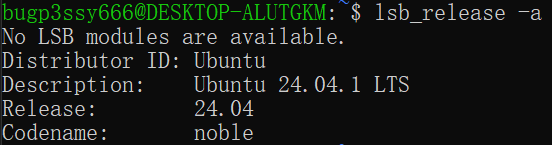
\includegraphics[width=0.6\linewidth]{sys.png}
    \caption{系统和发行版信息}
    \label{fig:placeholder}
\end{figure}

以及内核架构信息:
\begin{figure} [H]
    \centering
    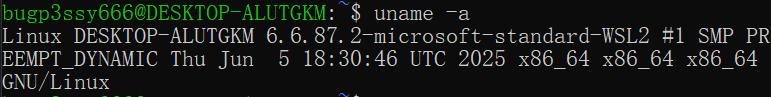
\includegraphics[width=0.75\linewidth]{struct.png}
    \caption{内核架构信息}
    \label{fig:placeholder}
\end{figure}

上图说明了本虚拟系统为在 Windows 的 WSL2 下运行的Linux内核;运行的 CPU 架构、内核架构、硬件平台类型均为“x86\_64”,即在 \textbf{64 位 x86 CPU 上运行 64 位内核};操作系统环境为\textbf{“GNU 工具链 + Linux 内核”}。



%——————————————————————————————————————
\vspace{3em}

\section{实验一:深入了解编译流程和编译器功能}
%——————————————————————————————————————
\subsection{总流程}
\begin{figure} [H]
    \centering
    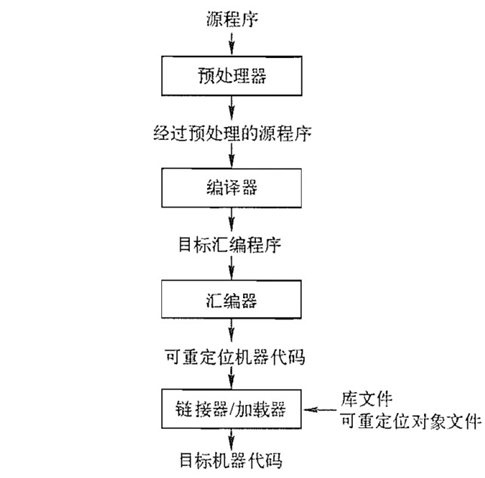
\includegraphics[width=0.7\linewidth]{the_whole_process_screenshot.png}
    \caption{完整编译流程图}
    \label{fig:placeholder}
\end{figure}
本课题研究C程序的编译过程,完整编译流程如上图所示。简要来说,每个阶段的主要作用如下:
\begin{enumerate}
    \item \textbf{预处理器:}处理源代码所有\textbf{以\texttt{\#}开头的预编译}指令(\texttt{\#include \#define \#if ...})
    \item \textbf{编译器:}将预处理后的C代码翻译成\textbf{汇编语言}。
    \item \textbf{汇编器:}将汇编语言指令翻译成\textbf{机器语言}指令,并将汇编语言程序打包成\textbf{可重定位的目标程序}。
    \item \textbf{链接器:}将可重定位的目标程序(可以是多个)引入\textbf{库文件},生成最终可运行的目标代码。
    \item \textbf{加载器:}加载资源文件到虚拟内存合适地址,预备启动程序。
\end{enumerate}

为了逐步验证各个阶段产生的作用,由实验提供的简单程序为出发点,作以下两点调整:
\begin{itemize}
    \item C语言不支持\texttt{cin, cout}等\textbf{输入输出流},将此类指令改为C语言适用的指令,如\texttt{printf(), scanf()}等等。
    \item 加入一些\textbf{预编译指令、注释},为预处理器阶段验证作补充。
\end{itemize}

\label{code1}

修改后的C语言代码如下所示:
\begin{lstlisting}[title=一个简单的斐波那契数列C程序,frame=trbl,language={C++}]
#include <stdio.h>

#define MAX_N 50
#define INIT_A 0
#define INIT_B 1

#define PRINT(x) printf("%d\n", x)

int main() {
    int a, b, i, t, n;

    a = INIT_A;
    b = INIT_B;
    i = 1;

    scanf("%d", &n);
    if (n > MAX_N) {
        printf("Input exceeds maximum value %d\n", MAX_N);
        return 1;
    }

    PRINT(a);
    PRINT(b);

    // this is a friendly annotation *
    while (i < n)
    {
        t = b;
        b = a + b;
        PRINT(b);
        a = t;
        i = i + 1;
    }
}
\end{lstlisting}

下面按照步骤编译,依次验证和探究各个步骤做了什么工作。

\vspace{1em}

\subsection{预处理器}
\subsubsection{预处理的具体功能}
\textbf{预处理}是 C/C++ 程序\textbf{从源代码到编译}的第一步。在这一阶段,编译器的预处理器(cpp)只处理 \texttt{\#} 开头的指令以及注释,对源代码进行文本级别的加工,生成一个“纯净”的源文件,交由编译器进行后续分析。

更加具体来说,其主要工作有:
\begin{enumerate}
    \item \textbf{头文件展开:} 处理 \texttt{\#include} 指令,把指定的头文件内容\textbf{直接拷贝}进来。
    \item \textbf{宏替换/宏展开:} 处理 \texttt{\#define} 定义的宏,其中对于\textbf{对象宏}将其用原先的简单文本替换掉,对于\textbf{函数宏}则用带参数的文本替换。
    \item \textbf{条件编译:} 根据条件来\textbf{选择性}编译所需要部分的代码,相关常见指令有 \texttt{\#if, \#ifdef, \#ifndef, \#elif, \#else, \#endif}.
    \item \textbf{注释删除:} 所有\texttt{/* ... */} 和 \texttt{// ...} 诸如此类的注释信息都会被删除,不进入编译阶段。
    \item \textbf{*其他处理:} 其他一些预处理指令的处理,如 \texttt{\#undef} 可以取消一个宏定义,\texttt{\#line} 指令可以改变编译器记录的行号和文件名,\texttt{\#error} 会强制在预处理时报错,\texttt{\#warning} 会发出警告(某些编译器支持),等等。
    \item \textbf{*特殊宏替换:} 由编译器提供的特殊宏替换,有\texttt{\_\_FILE\_\_, \_\_LINE\_\_, \_\_DATE\_\_, \_\_TIME\_\_}等,不作详细介绍。
\end{enumerate}

在本实验的研究当中,前四点作用是主要研究对象。

\subsubsection{进行预处理并验证功能}
在实验目录下终端中输入以下命令:

\begin{center}
    \textcolor{deepblue}{\textbf{\texttt{\large{gcc main.c -E -o main.i}}}}
\end{center}

对于该命令的理解是:添加参数\texttt{-E}让gcc\textbf{只进行预处理}过程;参数\texttt{-o}改变gcc输出文件名。\texttt{.i}是标准的预处理后源码文件格式。

执行命令后,观察到目录下新生成一个文件\texttt{main.i},说明预处理进行成功。打开进行其功能验证,其中发现:

\textbf{\textcircled{1}} 文件中出现诸多以下类型的代码段:
\begin{figure} [H]
    \centering
    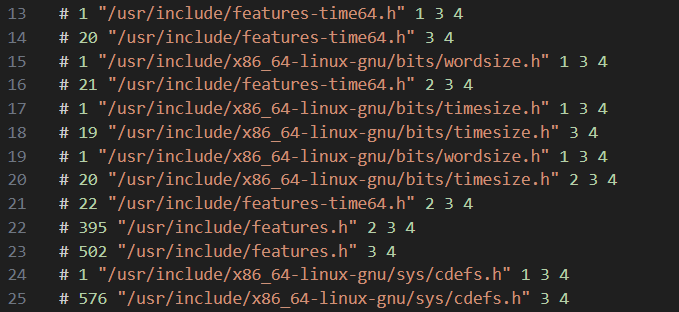
\includegraphics[width=0.70\linewidth]{cpp_1.png}
    \caption{预处理器插入的行控制指令}
    \label{fig:placeholder}
\end{figure} \label{pic2}

\begin{figure} [H]
    \centering
    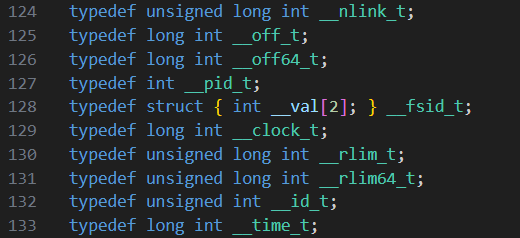
\includegraphics[width=0.70\linewidth]{cpp_2.png}
    \caption{大量定义类型别名的指令}
    \label{fig:placeholder}
\end{figure}

\begin{figure} [H]
    \centering
    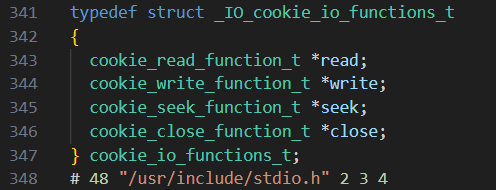
\includegraphics[width=0.70\linewidth]{cpp_3.png}
    \caption{结构体的定义与声明}
    \label{fig:placeholder}
\end{figure}

\begin{figure} [H]
    \centering
    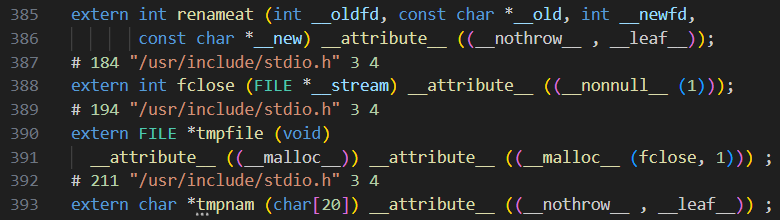
\includegraphics[width=0.70\linewidth]{cpp_4.png}
    \caption{各种函数体声明}
    \label{fig:placeholder}
\end{figure}

其中对于\hyperref[pic2]{\textcolor{deepblue}{图4}}的指令可以进一步分析:

\begin{center}
    \textcolor{deepred}{\textbf{\texttt{\# <行号> "<文件名>" <可选标志>}}}
\end{center}

其中\textbf{<行号>}告诉编译器“接下来的代码在源文件里属于哪一行”;\textbf{<文件名>}告诉编译器“这段代码来自哪个源文件”;而\textbf{<可选标志>}数字是一些特殊标记,用于区分文件种类和状态。其实\textbf{<行号>}信息在其他指令部分也都有出现。

以上几种代码段基本都来源于\texttt{\#include}头文件包含的处理,加之以对源代码的解读(涉及到行号信息的获取)。所有声明都是对头文件内容的直接或间接拷贝。这些声明占了约800行,可知\texttt{<stdio.h>}包还是很庞大的(包括其内部再引用别的头文件)。

\vspace{1em}

\textbf{\textcircled{2}} 在文件最后部分,出现了与原先C程序代码相似度很高的代码段:
\begin{lstlisting}[title=预处理后的C程序代码,frame=trbl,language={C++}]
# 9 "main.c"
int main() {
    int a, b, i, t, n;

    a = 0;
    b = 1;
    i = 1;

    scanf("%d", &n);
    if (n > 50) {
        printf("Input exceeds maximum value %d\n", 50);
        return 1;
    }

    printf("%d\n", a);
    printf("%d\n", b);


    while (i < n)
    {
        t = b;
        b = a + b;
        printf("%d\n", b);
        a = t;
        i = i + 1;
    }
}
\end{lstlisting}

这里出现了 \texttt{\# 9} 的行号信息,回到\hyperref[code1]{\textcolor{deepblue}{原始代码}}中,可以观察到\texttt{main}函数的确是从第9行开始的,可以验证行号信息的正确性。

综合分析这段代码,会发现是和原代码\textbf{逻辑一致且正确}的“简单斐波那契数列”程序,但有一些细节上的改变:
\begin{enumerate}
    \item \textbf{头文件引用消失:} 由上面的分析可知,头文件具体内容已经被全部拷贝至此文件前面部分,所以不再需要声明。
    \item \textbf{宏定义被替换:} 源代码中对参数初始值以及输出函数(\texttt{printf() -> PRINT()})进行了宏定义(\texttt{\#define}),主函数代码中直接使用替换符;而预处理后的代码删除了宏定义,且将替换符全部替换为原始数据或函数。
    \item \textbf{注释被删除:} 源代码添加了一行\texttt{// ...} 注释作为测试,在预处理后的代码中没有出现,说明注释被删除。
\end{enumerate}

这些变化和预处理的各项既定功能是相符合的,则\textbf{预处理器功能验证完毕}。

\vspace{1em}

\subsection{编译器}
编译过程是本课程着重学习和研究的过程。它接收\textbf{源代码}文件,输出\textbf{汇编代码}。其过程中主要完成的工作有:
\begin{itemize}
    \item \textbf{翻译:}将原来的高级语言代码翻译成机器能够进一步处理的\textbf{汇编代码}。
    \item \textbf{检查:}检查原先代码逻辑中的语法错误、语义错误并反馈。
    \item \textbf{优化:}改进程序结构或指令,使生成的代码运行更快或占用更少资源。
\end{itemize}

接下来逐步分析编译器处理各个阶段完成的工作。

\subsubsection{词法分析}
\texttt{\large{词法分析:主要工作是把源代码的字符流分割成\textbf{token序列}(关键字、标识符、常量、操作符、分隔符......),促进后续对于代码结构和语法的理解。}}

\vspace{1em}


进行词法分析仍从源C代码出发,执行以下命令:

\begin{center}
    \textcolor{deepblue}{\textbf{\texttt{\large{clang -E -Xclang -dump-tokens main.c}}}}
\end{center}

命令调用了Clang 编译器前端。其中参数\texttt{-E}依旧代表只进行预编译;参数\texttt{-Xclang}用来告诉 Clang 驱动程序,后面跟着的文件内容直接传给 Clang 前端,而非驱动器自己处理;\texttt{-dump-tokens}是核心意义的参数,它是 Clang 前端的一个内部调试选项,能够在\textbf{词法分析}阶段打印出\textbf{所有的token}.

词法分析的结果会直接在终端打印出来(当然也可以使用shell重定向,导出为文本文件),可以截取输出结果中的实际逻辑部分进行分析,探究其含义。

\vspace{1em}


\begin{lstlisting}[title=词法分析片段 1, frame=trbl,language={C++}]
int 'int'        [StartOfLine]  Loc=<main.c:9:1>
identifier 'main'        [LeadingSpace] Loc=<main.c:9:5>
l_paren '('             Loc=<main.c:9:9>
r_paren ')'             Loc=<main.c:9:10>
l_brace '{'      [LeadingSpace] Loc=<main.c:9:12>
\end{lstlisting}

这一片段对应源代码的:

\begin{lstlisting}[frame=trbl,language={C++}]
int main() {
\end{lstlisting}
这一行。\texttt{int}是\textbf{关键词token},直接被标记为“\texttt{int}”,而\texttt{[StartOfLine]}则表示这一关键词出现在该代码行之首(此标记不再说明),\texttt{Loc}段表示其在源代码文件中的\textbf{起始}具体位置,包括文件、行与列信息(例如,\texttt{Loc=<main.c:9:1>}表示此语句从\texttt{main.c}中第9行、第1列/第1个字符起始。此后,\texttt{Loc}的含义都如此,不再赘述)。对于\texttt{main},将其识别为\texttt{identifier},即\textbf{标识符},并且冠以\texttt{[LeadingSpace]}标记,说明前面有空格(此标记不再说明)。对于三个字符,\texttt{l\_paren, r\_paren, l\_brace}的token命名很直接,分别表示“左括号”“右括号”“左大括号”。

由上面的分析可知,一般对于一个token的分析结果有这几个组成成分:

\begin{center}
    \textcolor{deepred}{\textbf{\texttt{\textsuperscript{\textcircled{1}}token种类 + \textsuperscript{\textcircled{2}}'token内容' + \textsuperscript{\textcircled{3}}[附加信息标记(可选)] + \textsuperscript{\textcircled{4}}Loc=<源代码位置>}}}
\end{center}

有了以上的分析经验,不难将剩下的词法分析结果对应到相应的源代码:

\vspace{1em}

\begin{lstlisting}[title=词法分析片段 2,frame=trbl,language={C++}]
int 'int'        [StartOfLine] [LeadingSpace]   Loc=<main.c:10:5>
identifier 'a'   [LeadingSpace] Loc=<main.c:10:9>
comma ','               Loc=<main.c:10:10>
identifier 'b'   [LeadingSpace] Loc=<main.c:10:12>
comma ','               Loc=<main.c:10:13>
identifier 'i'   [LeadingSpace] Loc=<main.c:10:15>
comma ','               Loc=<main.c:10:16>
identifier 't'   [LeadingSpace] Loc=<main.c:10:18>
comma ','               Loc=<main.c:10:19>
identifier 'n'   [LeadingSpace] Loc=<main.c:10:21>
semi ';'                Loc=<main.c:10:22>
\end{lstlisting}

这一部分对应源代码的:
\begin{lstlisting}[frame=trbl,language={C++}]
    int a, b, i, t, n;
\end{lstlisting}
这一行,是声明全局变量的语句。其中新出现了\texttt{comma, semi}两个token,分别对应源码的逗号和分号分隔符。

\vspace{1em}


\begin{lstlisting}[title=词法分析片段 3,frame=trbl,language={C++}]
identifier 'a'   [StartOfLine] [LeadingSpace]   Loc=<main.c:12:5>
equal '='        [LeadingSpace] Loc=<main.c:12:7>
numeric_constant '0'     [LeadingSpace] Loc=<main.c:12:9 <Spelling=main.c:4:16>>
semi ';'                Loc=<main.c:12:15>
identifier 'b'   [StartOfLine] [LeadingSpace]   Loc=<main.c:13:5>
equal '='        [LeadingSpace] Loc=<main.c:13:7>
numeric_constant '1'     [LeadingSpace] Loc=<main.c:13:9 <Spelling=main.c:5:16>>
semi ';'                Loc=<main.c:13:15>
identifier 'i'   [StartOfLine] [LeadingSpace]   Loc=<main.c:14:5>
equal '='        [LeadingSpace] Loc=<main.c:14:7>
numeric_constant '1'     [LeadingSpace] Loc=<main.c:14:9>
semi ';'                Loc=<main.c:14:10>
\end{lstlisting}

这一部分对应源代码的:
\begin{lstlisting}[frame=trbl,language={C++}]
    a = INIT_A;
    b = INIT_B;
    i = 1;
\end{lstlisting}
这几行,对变量赋初值。等号/赋值号被表意地标记为\texttt{equal}.

值得注意的是,此处出现了\texttt{numeric\_constant}这个新token,和\texttt{Spelling}这个在\texttt{Loc}参数中出现的附属参数。显而易见的是\texttt{numeric\_constant}代表\textbf{数值常量},作为赋值式子中的右值是顺理成章的;而特别地对于\texttt{a, b}两参量中的\texttt{Spelling}从何而来,经过分析理解,是由于源代码中对于\texttt{a, b}两个参数的赋值使用了\textbf{宏定义}常量,所以并非像\texttt{i}的赋值一样直接使用常数,而是需要宏展开,\texttt{Spelling}标注的位置就是源代码中\textbf{宏定义声明}的位置。

\vspace{1em}

\begin{lstlisting}[title=词法分析片段 4,frame=trbl,language={C++}]
identifier 'scanf'       [StartOfLine] [LeadingSpace]   Loc=<main.c:16:5>
l_paren '('             Loc=<main.c:16:10>
string_literal '"%d"'           Loc=<main.c:16:11>
comma ','               Loc=<main.c:16:15>
amp '&'  [LeadingSpace] Loc=<main.c:16:17>
identifier 'n'          Loc=<main.c:16:18>
r_paren ')'             Loc=<main.c:16:19>
semi ';'                Loc=<main.c:16:20>
\end{lstlisting}

这一部分对应源代码的:
\begin{lstlisting}[frame=trbl,language={C++}]
    scanf("%d", &n);
\end{lstlisting}
这一行,接收用户输入整型数。出现了新的token,名为\texttt{string\_literal}和\texttt{amp},意义比较明确不再赘述。可以发现,函数和变量一样,只是宽泛地、默认地被标记为\texttt{identifier}.


\vspace{1em}


\begin{lstlisting}[title=词法分析片段 5,frame=trbl,language={C++}]
if 'if'  [StartOfLine] [LeadingSpace]   Loc=<main.c:17:5>
l_paren '('      [LeadingSpace] Loc=<main.c:17:8>
identifier 'n'          Loc=<main.c:17:9>
greater '>'      [LeadingSpace] Loc=<main.c:17:11>
numeric_constant '50'    [LeadingSpace] Loc=<main.c:17:13 <Spelling=main.c:3:15>>
r_paren ')'             Loc=<main.c:17:18>
l_brace '{'      [LeadingSpace] Loc=<main.c:17:20>
identifier 'printf'      [StartOfLine] [LeadingSpace]   Loc=<main.c:18:9>
l_paren '('             Loc=<main.c:18:15>
string_literal '"Input exceeds maximum value %d\n"'             Loc=<main.c:18:16>
comma ','               Loc=<main.c:18:50>
numeric_constant '50'    [LeadingSpace] Loc=<main.c:18:52 <Spelling=main.c:3:15>>
r_paren ')'             Loc=<main.c:18:57>
semi ';'                Loc=<main.c:18:58>
return 'return'  [StartOfLine] [LeadingSpace]   Loc=<main.c:19:9>
numeric_constant '1'     [LeadingSpace] Loc=<main.c:19:16>
semi ';'                Loc=<main.c:19:17>
r_brace '}'      [StartOfLine] [LeadingSpace]   Loc=<main.c:20:5>
\end{lstlisting}

这一部分对应源代码的:
\begin{lstlisting}[frame=trbl,language={C++}]
    if (n > MAX_N) {
        printf("Input exceeds maximum value %d\n", MAX_N);
        return 1;
    }
\end{lstlisting}
这几行,出现了与判断分支相关的新token。其中\texttt{if}关键词直接被标记为\texttt{if};判断语句中的大于号被标记为\texttt{greater}. 以及这里还出现了“满足条件直接结束程序”的\texttt{return}逻辑,能注意到\texttt{return}关键词也直接被标记为\texttt{return}. 此外,判断句中的常量再次使用到了宏定义,可以观察到\texttt{Spelling}照常出现。

\vspace{2em}


\begin{lstlisting}[title=词法分析片段 6,frame=trbl,language={C++}]
identifier 'printf'      [StartOfLine] [LeadingSpace]   Loc=<main.c:22:5 <Spelling=main.c:7:18>>
l_paren '('             Loc=<main.c:22:5 <Spelling=main.c:7:24>>
string_literal '"%d\n"'         Loc=<main.c:22:5 <Spelling=main.c:7:25>>
comma ','               Loc=<main.c:22:5 <Spelling=main.c:7:31>>
identifier 'a'   [LeadingSpace] Loc=<main.c:22:5 <Spelling=main.c:22:11>>
r_paren ')'             Loc=<main.c:22:5 <Spelling=main.c:7:34>>
semi ';'                Loc=<main.c:22:13>
identifier 'printf'      [StartOfLine] [LeadingSpace]   Loc=<main.c:23:5 <Spelling=main.c:7:18>>
l_paren '('             Loc=<main.c:23:5 <Spelling=main.c:7:24>>
string_literal '"%d\n"'         Loc=<main.c:23:5 <Spelling=main.c:7:25>>
comma ','               Loc=<main.c:23:5 <Spelling=main.c:7:31>>
identifier 'b'   [LeadingSpace] Loc=<main.c:23:5 <Spelling=main.c:23:11>>
r_paren ')'             Loc=<main.c:23:5 <Spelling=main.c:7:34>>
semi ';'                Loc=<main.c:23:13>
\end{lstlisting}

这一部分对应源代码的:
\begin{lstlisting}[frame=trbl,language={C++}]
    PRINT(a);
    PRINT(b);
\end{lstlisting}
这两行,输出\texttt{a, b}的值。此处使用到了\textbf{函数的宏定义},所以在经过两个函数体的时候都用\texttt{Spelling}标记了宏定义声明所在的源码位置。

\vspace{1em}


\begin{lstlisting}[title=词法分析片段 7,frame=trbl,language={C++}]
while 'while'    [StartOfLine] [LeadingSpace]   Loc=<main.c:26:5>
l_paren '('      [LeadingSpace] Loc=<main.c:26:11>
identifier 'i'          Loc=<main.c:26:12>
less '<'         [LeadingSpace] Loc=<main.c:26:14>
identifier 'n'   [LeadingSpace] Loc=<main.c:26:16>
r_paren ')'             Loc=<main.c:26:17>
l_brace '{'      [StartOfLine] [LeadingSpace]   Loc=<main.c:27:5>
identifier 't'   [StartOfLine] [LeadingSpace]   Loc=<main.c:28:9>
equal '='        [LeadingSpace] Loc=<main.c:28:11>
identifier 'b'   [LeadingSpace] Loc=<main.c:28:13>
semi ';'                Loc=<main.c:28:14>
identifier 'b'   [StartOfLine] [LeadingSpace]   Loc=<main.c:29:9>
equal '='        [LeadingSpace] Loc=<main.c:29:11>
identifier 'a'   [LeadingSpace] Loc=<main.c:29:13>
plus '+'         [LeadingSpace] Loc=<main.c:29:15>
identifier 'b'   [LeadingSpace] Loc=<main.c:29:17>
semi ';'                Loc=<main.c:29:18>
identifier 'printf'      [StartOfLine] [LeadingSpace]   Loc=<main.c:30:9 <Spelling=main.c:7:18>>
l_paren '('             Loc=<main.c:30:9 <Spelling=main.c:7:24>>
string_literal '"%d\n"'         Loc=<main.c:30:9 <Spelling=main.c:7:25>>
comma ','               Loc=<main.c:30:9 <Spelling=main.c:7:31>>
identifier 'b'   [LeadingSpace] Loc=<main.c:30:9 <Spelling=main.c:30:15>>
r_paren ')'             Loc=<main.c:30:9 <Spelling=main.c:7:34>>
semi ';'                Loc=<main.c:30:17>
identifier 'a'   [StartOfLine] [LeadingSpace]   Loc=<main.c:31:9>
equal '='        [LeadingSpace] Loc=<main.c:31:11>
identifier 't'   [LeadingSpace] Loc=<main.c:31:13>
semi ';'                Loc=<main.c:31:14>
identifier 'i'   [StartOfLine] [LeadingSpace]   Loc=<main.c:32:9>
equal '='        [LeadingSpace] Loc=<main.c:32:11>
identifier 'i'   [LeadingSpace] Loc=<main.c:32:13>
plus '+'         [LeadingSpace] Loc=<main.c:32:15>
numeric_constant '1'     [LeadingSpace] Loc=<main.c:32:17>
semi ';'                Loc=<main.c:32:18>
r_brace '}'      [StartOfLine] [LeadingSpace]   Loc=<main.c:33:5>
\end{lstlisting}

这一部分对应源代码的:
\begin{lstlisting}[frame=trbl,language={C++}]
    while (i < n)
    {
        t = b;
        b = a + b;
        PRINT(b);
        a = t;
        i = i + 1;
    }
\end{lstlisting}
这几行,是进行斐波那契数列计算的循环体。\texttt{while}循环关键词被直接标记为\texttt{while};小于号被标记为\texttt{less},加号被标记为\texttt{plus}. 其他内容在前面均有出现。

\vspace{1em}


\begin{lstlisting}[title=词法分析片段 8,frame=trbl,language={C++}]
r_brace '}'      [StartOfLine]  Loc=<main.c:34:1>
eof ''          Loc=<main.c:34:2>
\end{lstlisting}

这是程序的结尾,一个是主函数域的右括号,还有一个\texttt{eof}标识符用于表示\textbf{程序的结束}。

\vspace{1em}

综合观察以上的词法分析结果,发现并没有出现源代码中的\textbf{头文件声明}、\textbf{宏定义}、\textbf{注释},或被替换或被删除。这说明,词法分析之前,编译器已经完成了预处理所做的所有工作,这也间接说明了之前分析的\texttt{-E}命令参数的实际作用。

当然,一切头文件引用也被包含在词法分析中并罗列在主程序的分析之前,但太过冗杂且基本逻辑是一致的,便不再分析。

\vspace{1em}

至此,编译器的\textbf{词法分析阶段功能验证完毕}。

\subsubsection{语法分析}
\texttt{\large{语法分析:主要工作是根据语言语法把 token 序列组织成\textbf{语法树}(Parse Tree)或\textbf{抽象语法树}(AST/Abstract Syntax Tree)。
它在生成语法树的同时,还能检查并产生\textbf{语法错误}信息,以及做初步的\textbf{结构检查}。}}

\vspace{1em}

进行语法分析依旧从源C代码出发,执行以下命令:
\begin{center}
    \textcolor{deepblue}{\textbf{\texttt{\large{clang -E -Xclang -ast-dump main.c}}}}
\end{center}

命令基本构成和调用方法和词法分析基本相同。其中核心意义参数\texttt{-ast-dump}替换词法分析中的\texttt{-dump-tokens},它能够是在\textbf{语法分析}阶段打印出完整的\textbf{AST抽象语法树}。

在终端,直接输出AST抽象语法树的效果如下图所示:
\begin{figure} [H]
    \centering
    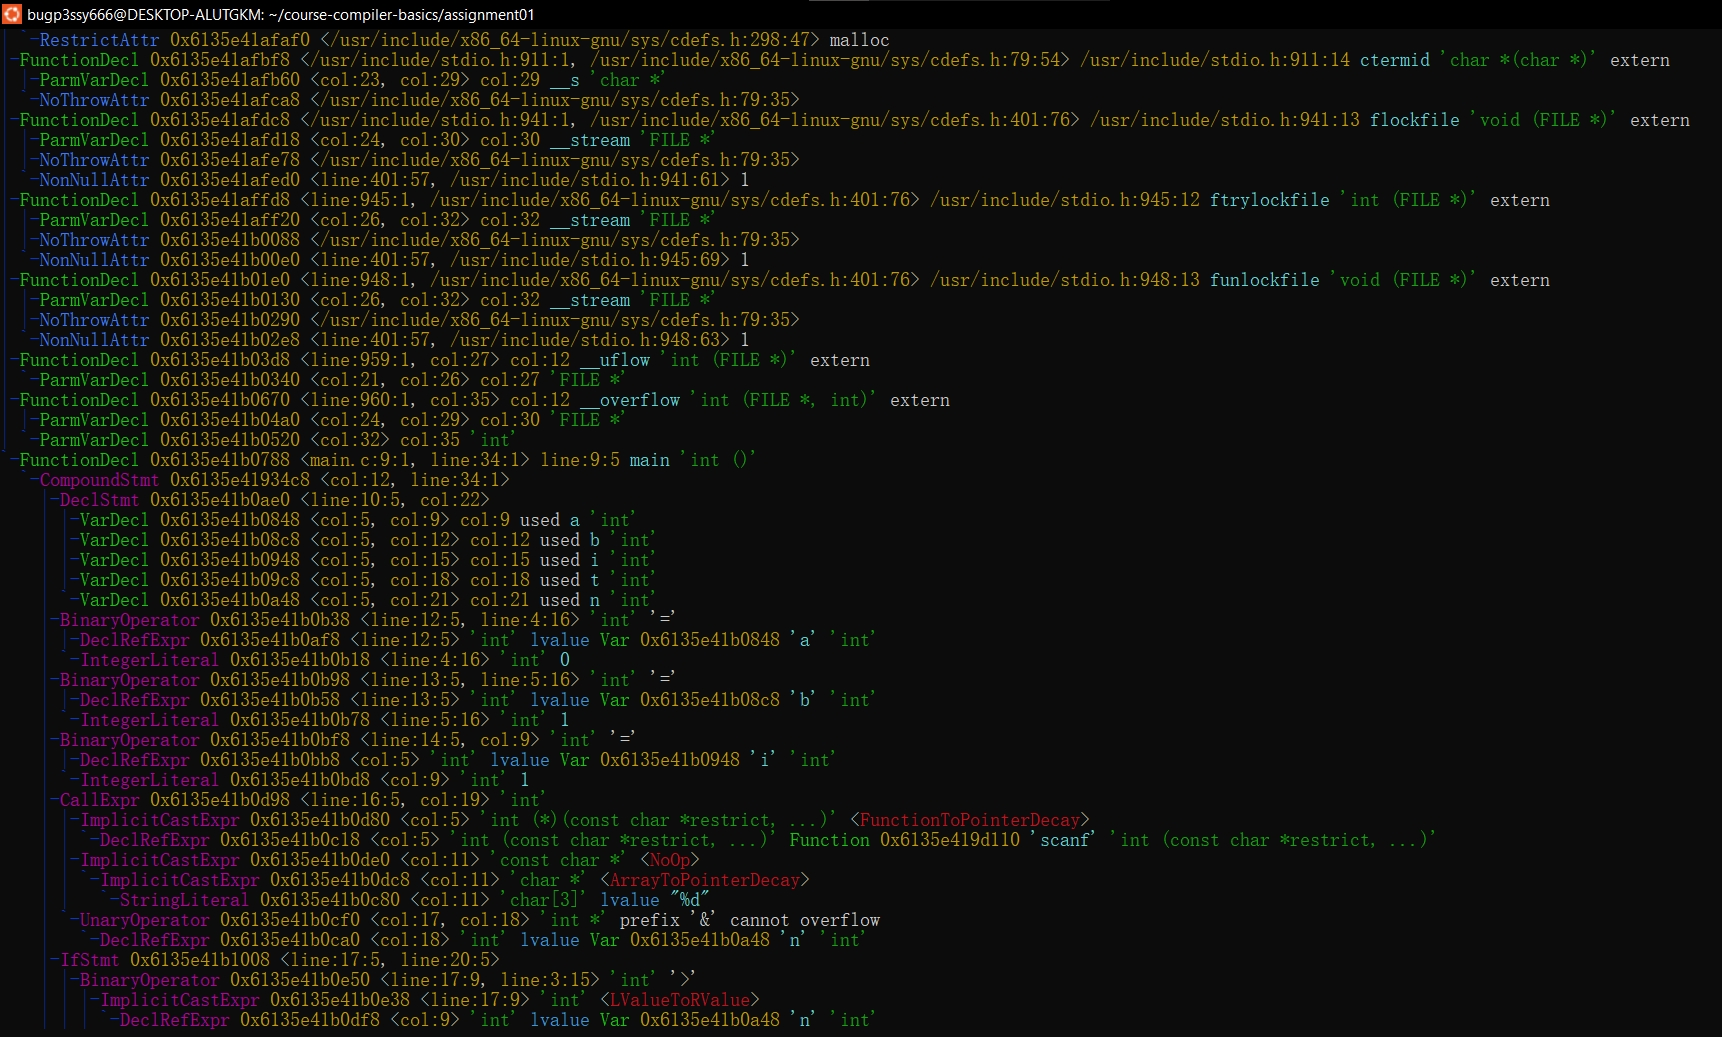
\includegraphics[width=0.9\linewidth]{ccl_1.png}
    \caption{在Ubuntu终端直接输出AST}
    \label{fig:placeholder}
\end{figure}

下面对输出的AST树进行分析。整个AST(包括库文件引用)结构是很繁杂的,为缩减报告篇幅,在下面的分析中适当省略部分分支内容。

首先跳过库文件拷贝部分,找到\texttt{main}函数入口:
\begin{lstlisting}[frame=trbl,language={C++}]
-FunctionDecl 0x6423345a9718 <main.c:9:1, line:34:1> line:9:5 main 'int ()'
\end{lstlisting}

下面选取一些语句进行AST分析。

对于这一声明语句:
\begin{lstlisting}[frame=trbl,language={C++}]
    int a, b, i, t, n;
\end{lstlisting}
可以找到对应的AST片段:
\begin{lstlisting}[title=AST片段 1,frame=trbl]
-FunctionDecl 0x6135e41b0788 <main.c:9:1, line:34:1> line:9:5 main 'int ()'
  -CompoundStmt 0x6135e41934c8 <col:12, line:34:1>
    |-DeclStmt 0x6135e41b0ae0 <line:10:5, col:22>
    | |-VarDecl 0x6135e41b0848 <col:5, col:9> col:9 used a 'int'
    | |-VarDecl 0x6135e41b08c8 <col:5, col:12> col:12 used b 'int'
    | |-VarDecl 0x6135e41b0948 <col:5, col:15> col:15 used i 'int'
    | |-VarDecl 0x6135e41b09c8 <col:5, col:18> col:18 used t 'int'
    |  -VarDecl 0x6135e41b0a48 <col:5, col:21> col:21 used n 'int'
\end{lstlisting}

首先看各个节点的命名。第一行是\texttt{main}函数入口,标记为\texttt{FunctionDecl},即“函数声明”,也可以视为主程序的\textbf{根节点}。下面第一级子节点标记为\texttt{CompoundStmt},意为“\textbf{复合语句块}”,代表这一整个层级。再下一级节点标记为\texttt{DeclStmt},意为“\textbf{声明语句}”,说明这一复合语句的具体类型和作用。最低一级节点为若干\texttt{VarDecl},意为“变量声明”,每个节点对应原声明语句中的一个变量——\texttt{a, b, i, t, n}共5个变量,对应5个节点。

再看节点名后的两个(/段)参数。第一个\texttt{0x...}是对应变量或函数在当前程序中的指针地址;第二段参数与代码在文本中的位置有关,具体编写/含义各不相同。比如,对于\texttt{main}函数,\texttt{<main.c:9:1, line:34:1>}的含义是“函数从第 9 行第 1 列开始,到第 34 行第 1 列结束”,\texttt{line:9:5}的含义是其在源代码中的具体位置,即第9行第5个字符开始。而对于\texttt{CompoundStmt}和\texttt{DeclStmt}节点,其参数构成相近,尖括号内的前一参数表示语句开始位置,后一参数表示语句结束位置。最后,对于\texttt{VarDecl}节点,有三个\texttt{col}参数,第一个是所属语句的开始列位置,第二个是此变量开始列位置,第三个是此变量结束列位置。由于上面例句中变量都只有一个字符长度,所以后两个参数自然是一致的。

最后还可以观察到变量声明有几个额外参数。\texttt{used}表示该变量在整个程序中被使用过;后一个参数是变量名称;最后一个变量声明变量类型。

可见,AST除了包含基础的程序语法结构信息,还需包含每个语句中的位置、范围、名称、状态等信息,细致到单个变量或函数,整体信息丰富而完善。

\vspace{1em}

同理,还可以再对若干语句进行AST对应的分析。

再选择一个判断语句进行分析。以这个判断输入是否越界的判断语句块为例:
\begin{lstlisting}[frame=trbl,language={C++}]
if (n > MAX_N) {
    printf("Input exceeds maximum value %d\n", MAX_N);
    return 1;
}
\end{lstlisting}
找到对应的AST片段:
\begin{lstlisting}[title=AST片段 2,frame=trbl]
-FunctionDecl 0x6135e41b0788 <main.c:9:1, line:34:1> line:9:5 main 'int ()'
  -CompoundStmt 0x6135e41934c8 <col:12, line:34:1>
    |- ··· ··· ··· ···
    |-IfStmt 0x6135e41b1008 <line:17:5, line:20:5>
    | |-BinaryOperator 0x6135e41b0e50 <line:17:9, line:3:15> 'int' '>'
    | | |-ImplicitCastExpr 0x6135e41b0e38 <line:17:9> 'int' <LValueToRValue>
    | | |  -DeclRefExpr 0x6135e41b0df8 <col:9> 'int' lvalue Var 0x6135e41b0a48 'n' 'int'
    | |  -IntegerLiteral 0x6135e41b0e18 <line:3:15> 'int' 50
    |  -CompoundStmt 0x6135e41b0fe8 <line:17:20, line:20:5>
    |   |-CallExpr 0x6135e41b0f58 <line:18:9, col:57> 'int'
    |   | |-ImplicitCastExpr 0x6135e41b0f40 <col:9> 'int (*)(const char *, ...)' <FunctionToPointerDecay>
    |   | |  -DeclRefExpr 0x6135e41b0e70 <col:9> 'int (const char *, ...)' Function 0x6135e41713b8 'printf' 'int (const char *, ...)'
    |   | |-ImplicitCastExpr 0x6135e41b0fa0 <col:16> 'const char *' <NoOp>
    |   | |  -ImplicitCastExpr 0x6135e41b0f88 <col:16> 'char *' <ArrayToPointerDecay>
    |   | |    -StringLiteral 0x6135e41b0ed0 <col:16> 'char[32]' lvalue "Input exceeds maximum value %d\n"
    |   |  -IntegerLiteral 0x6135e41b0f08 <line:3:15> 'int' 50
    |    -ReturnStmt 0x6135e41b0fd8 <line:19:9, col:16>
    |      -IntegerLiteral 0x6135e41b0fb8 <col:16> 'int' 1
\end{lstlisting}

可以发现,代表判断语句块的\texttt{IfStmt}节点和上面分析的\texttt{DeclStmt}声明语句在AST是同级别的,因为他们都是在\texttt{main}函数中最外一层的语句。

第一步,详细分析一下这个条件表达式:
\begin{lstlisting}[frame=trbl]
    |-IfStmt ··· ···
    | |-BinaryOperator 0x6135e41b0e50 <line:17:9, line:3:15> 'int' '>'
    | | |-ImplicitCastExpr 0x6135e41b0e38 <line:17:9> 'int' <LValueToRValue>
    | | |  -DeclRefExpr 0x6135e41b0df8 <col:9> 'int' lvalue Var 0x6135e41b0a48 'n' 'int'
    | |  -IntegerLiteral 0x6135e41b0e18 <line:3:15> 'int' 50
\end{lstlisting}

\label{implicit-expr}顶层\texttt{BinaryOperator}节点是识别二元操作符“>”大于号的结果,同时也划定了这个语句的类型。下一级节点有两个,左操作数是\texttt{ImplicitCastExpr}即\textbf{隐式转换表达式},后标注了\texttt{<LValueToRValue>},含义是将左值转化为右值,具体转化了什么参量稍后说明;右操作数是\texttt{IntegerLiteral}即\textbf{字面常量},这里是整数50. 其中左操作数还拥有再下一级的节点\texttt{DeclRefExpr},引用了局部变量\texttt{n},上面提到的左值转化为右值就是将这个变量的值转化为右值,才能够进行大小比较。

紧接着\texttt{BinaryOperator}节点之后顺接了同级的\texttt{CompoundStmt}节点,代表判断语句块的主体部分(大括号包括的部分)。

\texttt{CompoundStmt}节点下的主要部分是对\texttt{printf()}函数的调用:
\begin{lstlisting}[frame=trbl]
    | |  - ··· ··· ··· ···
    |  -CompoundStmt 0x6135e41b0fe8 <line:17:20, line:20:5>
    |   |-CallExpr 0x6135e41b0f58 <line:18:9, col:57> 'int'
    |   | |-ImplicitCastExpr 0x6135e41b0f40 <col:9> 'int (*)(const char *, ...)' <FunctionToPointerDecay>
    |   | |  -DeclRefExpr 0x6135e41b0e70 <col:9> 'int (const char *, ...)' Function 0x6135e41713b8 'printf' 'int (const char *, ...)'
    |   | |-ImplicitCastExpr 0x6135e41b0fa0 <col:16> 'const char *' <NoOp>
    |   | |  -ImplicitCastExpr 0x6135e41b0f88 <col:16> 'char *' <ArrayToPointerDecay>
    |   | |    -StringLiteral 0x6135e41b0ed0 <col:16> 'char[32]' lvalue "Input exceeds maximum value %d\n"
    |   |  -IntegerLiteral 0x6135e41b0f08 <line:3:15> 'int' 50
\end{lstlisting}

顶层\texttt{CallExpr}节点表示\textbf{函数调用},且注明了函数返回类型为\texttt{int}. 下一级节点的第一个比较特殊,是\texttt{<FunctionToPointerDecay>},即“函数名衰减为指针”,的隐式转换,这是C语言进行函数调用时为了让函数调用合法,自动插入的\textbf{函数名→函数指针转换}既定操作(转换后形如\texttt{int (*)(const char *, ...)}指向函数的指针)。后两个同级节点易于理解,是函数中的两个传参,分别对应字符串和常量。

其中字符串参数下属节点较多,着重分析一下。第一层,\texttt{ImplicitCastExpr <NoOp>},只作\textbf{类型微调},具体是\textbf{加\texttt{const}},NoOp 表示“不改变值,只做类型调整”。第二层,\texttt{ImplicitCastExpr <ArrayToPointerDecay>},将\textbf{数组衰减为指针},这同样来源于C语言的语法规则。第三层,\texttt{StringLiteral}来到字符串的实际内容。

\vspace{1em}

更多AST分析基本原理相似,不再赘述。编译器的\textbf{语法分析阶段功能验证完毕}。

\subsubsection{语义分析}
\texttt{\large{语义分析:主要工作是在 AST 上做\textbf{语义检查}并收集必要信息(类型、作用域、符号表)。换句话说,这一过程需要\textbf{理解程序的含义}并检查正确性,而\textbf{不仅仅是结构}。}}

\vspace{1em}

具体而言,语义分析所做的任务有:
\begin{itemize}
    \item \textbf{类型检查:} 确保操作数和操作符匹配,以及检查函数调用参数类型是否与函数定义匹配。这步也涉及\textbf{隐式类型转换},前面的\hyperref[implicit-expr]{\textcolor{deepblue}{\textbf{语法分析}}}阶段中有所提及。
    \item \textbf{检查标识符:} 确保每个变量和函数在使用前已经声明并检查是否重复定义。确保每个标识符(变量、函数、类型等)在正确作用域内调用。
    \item \textbf{函数调用检查:} 检查参数个数、参数类型是否匹配,检查返回类型是否正确。
    \item \textbf{常量表达式求值:} 对常量表达式做计算,生成\textbf{常量折叠}。
    \item \textbf{检查控制流语义:} 检查 \texttt{break, continue} 等是否在循环内部,\texttt{return}语句类型是否匹配函数返回类型。
    \item \textbf{构造和维护符号表:} 记录每个变量、函数、类型的属性信息,为作用域嵌套和查找提供支持。生成的符号表会用于后续步骤——\textbf{中间代码生成}和\textbf{优化}。
\end{itemize}

最重要的是类型检查、标识符检查和符号表的管理。

\vspace{1em}

语义分析没有提供具体的参考命令进行研究,以上是对于语义分析阶段的全部论述。

\subsubsection{中间代码生成}
中间代码生成:主要工作是把语义正确的 AST 翻译成一个与机器无关、便于优化的中间表示(IR)。

\vspace{1em}

中间代码的生成依旧从源C代码出发,首先执行以下命令来直接生成中间代码文件:
\begin{center}
    \textcolor{deepblue}{\textbf{\texttt{\large{clang -S -emit-llvm main.c}}}}
\end{center}

命令仍然使用Clang前端,其中\texttt{-S}参数表示只生成汇编/IR,不做汇编成目标文件;\texttt{-emit-llvm}参数告诉 Clang 不要生成本地汇编,而是生成 LLVM IR. 两者一并使用时,输出文件是 \texttt{.ll}格式文件(LLVM IR 文本形式);若不添加\texttt{-S}参数,输出的是 \texttt{.bc}格式文件(LLVM bitcode 二进制文件)。\label{we-talked-about-it-here}

执行命令后得到\texttt{main.ll}. 对于该文件,分段进行分析。


\begin{lstlisting}[title=main.ll 段落 1,frame=trbl,language={C++}]
; ModuleID = 'main.c'
source_filename = "main.c"
target datalayout = "e-m:e-p270:32:32-p271:32:32-p272:64:64-i64:64-i128:128-f80:128-n8:16:32:64-S128"
target triple = "x86_64-pc-linux-gnu"
\end{lstlisting}

这一段为\textbf{模块基本信息和目标平台设置}。其中\texttt{ModuleID}为模块标识符,此时为\texttt{main.c}. 源文件名同名。\texttt{target datalayout}和\texttt{target triple}描述数据在目标平台的布局和目标平台三元组(CPU架构-供应商-操作系统)。

\begin{lstlisting}[title=main.ll 段落 2,frame=trbl,language={C++}]
@.str = private unnamed_addr constant [3 x i8] c"%d\00", align 1
@.str.1 = private unnamed_addr constant [32 x i8] c"Input exceeds maximum value %d\0A\00", align 1
@.str.2 = private unnamed_addr constant [4 x i8] c"%d\0A\00", align 1
\end{lstlisting}

这一段定义 C 语言\textbf{字符串常量},供 \texttt{scanf/printf} 使用。其中\texttt{[N x i8]}代表长度为 N 的字符数组;\texttt{\textbackslash00} 为C字符串结尾;\texttt{private unnamed\_addr} 表示内部链接,LLVM 可优化地址访问。

\begin{lstlisting}[title=main.ll 段落 3,frame=trbl,language={C++}]
define dso_local i32 @main() #0 { ··· ··· }
\end{lstlisting}

主函数入口。有标明返回类型和函数属性。

\begin{lstlisting}[title=main.ll 段落 4,frame=trbl,language={C++}]
%1 = alloca i32, align 4
%2 = alloca i32, align 4
··· ··· ··· ···
%6 = alloca i32, align 4
\end{lstlisting}

这一段进行\textbf{栈空间的分配},\texttt{alloca}是分配栈上局部变量的指令。

\begin{lstlisting}[title=main.ll 段落 5,frame=trbl,language={C++}]
store i32 0, ptr %1, align 4
store i32 0, ptr %2, align 4
store i32 1, ptr %3, align 4
store i32 1, ptr %4, align 4
\end{lstlisting}

这一段给变量\textbf{赋初值},可对应到C语言代码:
\begin{lstlisting}[frame=trbl,language={C}]
a = 0; b = 0; i = 1; t = 1;
\end{lstlisting}


\begin{lstlisting}[title=main.ll 段落 6,frame=trbl,language={C++}]
%7 = call i32 (ptr, ...) @__isoc99_scanf(ptr noundef @.str, ptr noundef %6)
%8 = load i32, ptr %6, align 4
%9 = icmp sgt i32 %8, 50
br i1 %9, label %10, label %12
\end{lstlisting}

这一段进行输入数据越界检查(大小比较\textbf{判断语句})。前两行调用\texttt{scanf()}读取用户输入的\texttt{n}参数大小,第三行\texttt{icmp sgt}比较\texttt{n > 50 ?},最后一行进行条件跳转——判断语句为真,则跳转到\texttt{\%10}输出提示并终止,否则跳到 \texttt{\%12} 执行后续逻辑。具体\texttt{\%10}和\texttt{\%12}内容如何,下面将分析。根据阅读推测,他们应该代表预处理过后主程序代码的行号。


\begin{lstlisting}[title=main.ll 段落 7,frame=trbl,language={C++}]
10:                                               ; preds = %0
  %11 = call i32 (ptr, ...) @printf(ptr noundef @.str.1, i32 noundef 50)
  store i32 1, ptr %1, align 4
  br label %31
\end{lstlisting}

这是\texttt{\%10}的实际所指,\textbf{处理越界}情况。第一行输出越界提示,而后设置返回值为1,最后跳转(主函数返回)到\texttt{\%31}结束程序。

\begin{lstlisting}[title=main.ll 段落 8,frame=trbl,language={C++}]
12:                                               ; preds = %0
  %13 = load i32, ptr %2, align 4
  %14 = call i32 (ptr, ...) @printf(ptr noundef @.str.2, i32 noundef %13)
  ··· ··· ··· ···
  br label %17
17:                                               ; preds = %21, %12
  %18 = load i32, ptr %4, align 4
  ··· ··· ··· ···
  br i1 %20, label %21, label %31
21:                                               ; preds = %17
  %22 = load i32, ptr %3, align 4
  store i32 %22, ptr %5, align 4
  ··· ··· ··· ···
  store i32 %30, ptr %4, align 4
  br label %17, !llvm.loop !6
\end{lstlisting}

\texttt{12:}是前面\texttt{\%12}的实际所指。在这之后实际上就是\textbf{斐波那契数列计算}的核心逻辑,llvm代码较为冗长,所以不再逐行解析。

\begin{lstlisting}[title=main.ll 段落 9,frame=trbl,language={C++}]
31:                                               ; preds = %10, %17
  %32 = load i32, ptr %1, align 4
  ret i32 %32
\end{lstlisting}

之前提到过的\texttt{\%31}主程序返回逻辑所指。

\begin{lstlisting}[title=main.ll 段落 10,frame=trbl,language={C++}]
declare i32 @__isoc99_scanf(ptr noundef, ...) #1
declare i32 @printf(ptr noundef, ...) #1
\end{lstlisting}

这里是\textbf{外部函数声明},声明了 \texttt{scanf} 和 \texttt{printf},包括参数和返回类型等信息。

\begin{lstlisting}[title=main.ll 段落 11,frame=trbl,language={C++}]
attributes #0 = { noinline nounwind optnone uwtable ··· ··· }
attributes #1 = { ··· ··· }
\end{lstlisting}

这里规定了\textbf{函数属性}。其中\texttt{\#0}规定主函数属性,\texttt{\#1}规定外部函数属性。

\begin{lstlisting}[title=main.ll 段落 12,frame=trbl,language={C++}]
!llvm.module.flags = !{!0, !1, !2, !3, !4}
!llvm.ident = !{!5}

!0 = !{i32 1, !"wchar_size", i32 4}
!1 = !{i32 8, !"PIC Level", i32 2}
··· ··· ··· ···
!7 = !{!"llvm.loop.mustprogress"}
\end{lstlisting}

最后是\textbf{LLVM Metadata},包含存储编译器、循环属性等信息,用于优化和调试,不影响程序逻辑。

\vspace{1em}

除了直接生成LLVM IR文本文件,还可以添加命令参数(gcc flag)获得中间代码生成的多阶段的输出。执行下面的命令:
\begin{center}
    \textcolor{deepblue}{\textbf{\texttt{\large{gcc -O0 -fdump-tree-all-graph -fdump-rtl-all-graph main.c -o main}}}}
\end{center}

和前面不一样的是,这里使用了GNU编译器。\texttt{-O0}限定了优化保持关闭状态,方便完整地分析;\texttt{-fdump-tree-all-graph}能够输出 GCC 所有阶段的中间树表示(包括:GIMPLE/简化的三地址码表示,CFG/控制流图,SSA/静态单赋值形式),输出\texttt{.dot}格式的Graphviz文件;\texttt{-fdump-rtl-all-graph}能够输出所有阶段的 RTL(Register Transfer Level,中间寄存器表示),同样生成Graphviz可视化文件。

执行命令之后,可以看到目录中生成了有约百条记录:
\begin{figure}[htbp]
  \centering
  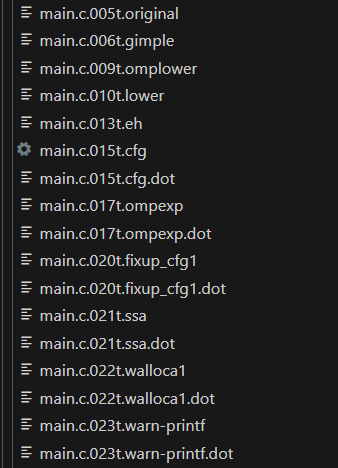
\includegraphics[height=6cm]{ccl_2.png}
  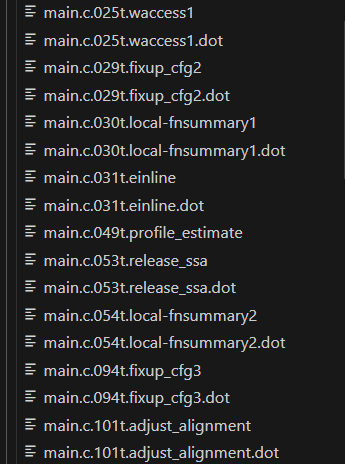
\includegraphics[height=6cm]{ccl_3.png}
  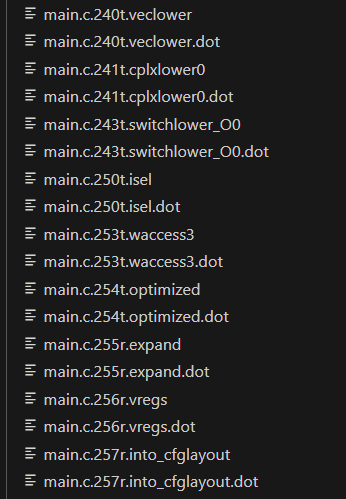
\includegraphics[height=6cm]{ccl_4.png}
  \caption{部分记录}
\end{figure}

简而言之,这些记录是GCC中间优化/分析阶段的 dump 文件。后缀为't'的命名段中的数字代表的就是阶段编号。

找出其中后缀为\texttt{cfg.dot}的文件:

\begin{center}
    
\texttt{\large{main.c.015t.cfg.dot}}

\texttt{\large{main.c.020t.fixup\_cfg1.dot}}

\texttt{\large{main.c.029t.fixup\_cfg2.dot}}

\texttt{\large{main.c.094t.fixup\_cfg3.dot}}

\end{center}

分别执行下面的命令:

\begin{center}
    \textcolor{deepblue}{\textbf{\texttt{\large{dot -Tpng main.c.015t.cfg.dot -o cfg01.png}}}}
\end{center}

\begin{center}
    \textcolor{deepblue}{\textbf{\texttt{\large{dot -Tpng main.c.020t.fixup\_cfg1.dot -o cfg02.png}}}}
\end{center}

\begin{center}
    \textcolor{deepblue}{\textbf{\texttt{\large{dot -Tpng main.c.029t.fixup\_cfg2.dot -o cfg03.png}}}}
\end{center}

\begin{center}
    \textcolor{deepblue}{\textbf{\texttt{\large{dot -Tpng main.c.094t.fixup\_cfg3.dot -o cfg04.png}}}}
\end{center}

就可以生成出一系列的\textbf{控制流图} (CFG)。这些流程图的变化,一定程度上反映了程序结构随着优化/分析而向着精简与高效进步的过程。

\begin{figure} [H]
    \centering
    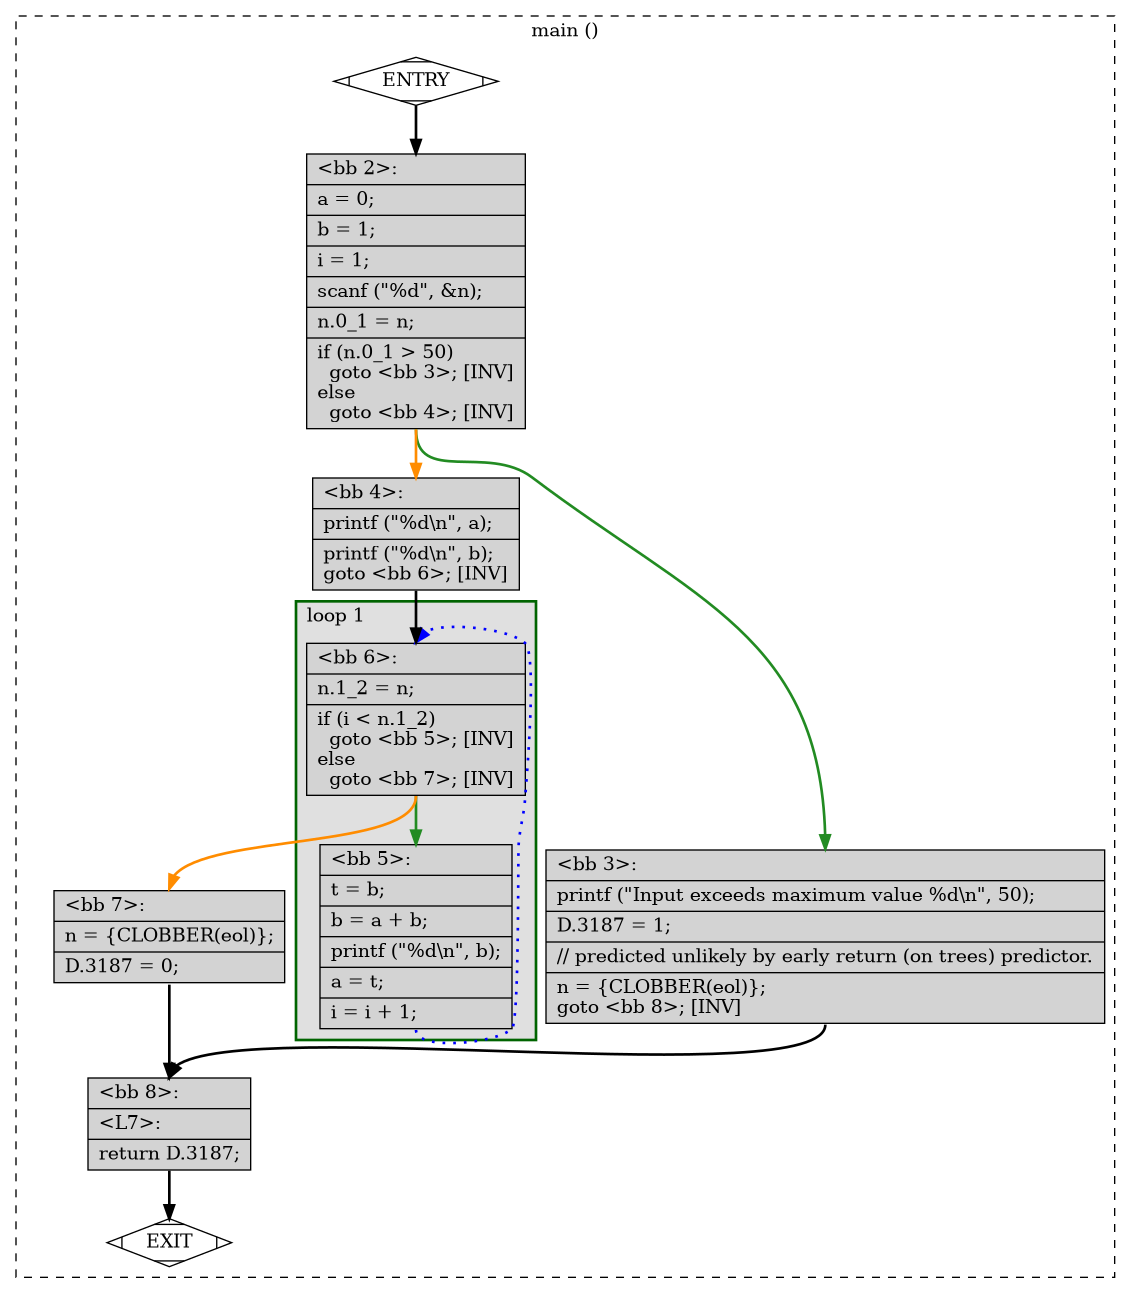
\includegraphics[width=0.5\linewidth]{ccl_5.png}
    \caption{cfg01.png/cfg02.png (015t/020t)}
    \label{fig:placeholder}
\end{figure}

\begin{figure} [H]
    \centering
    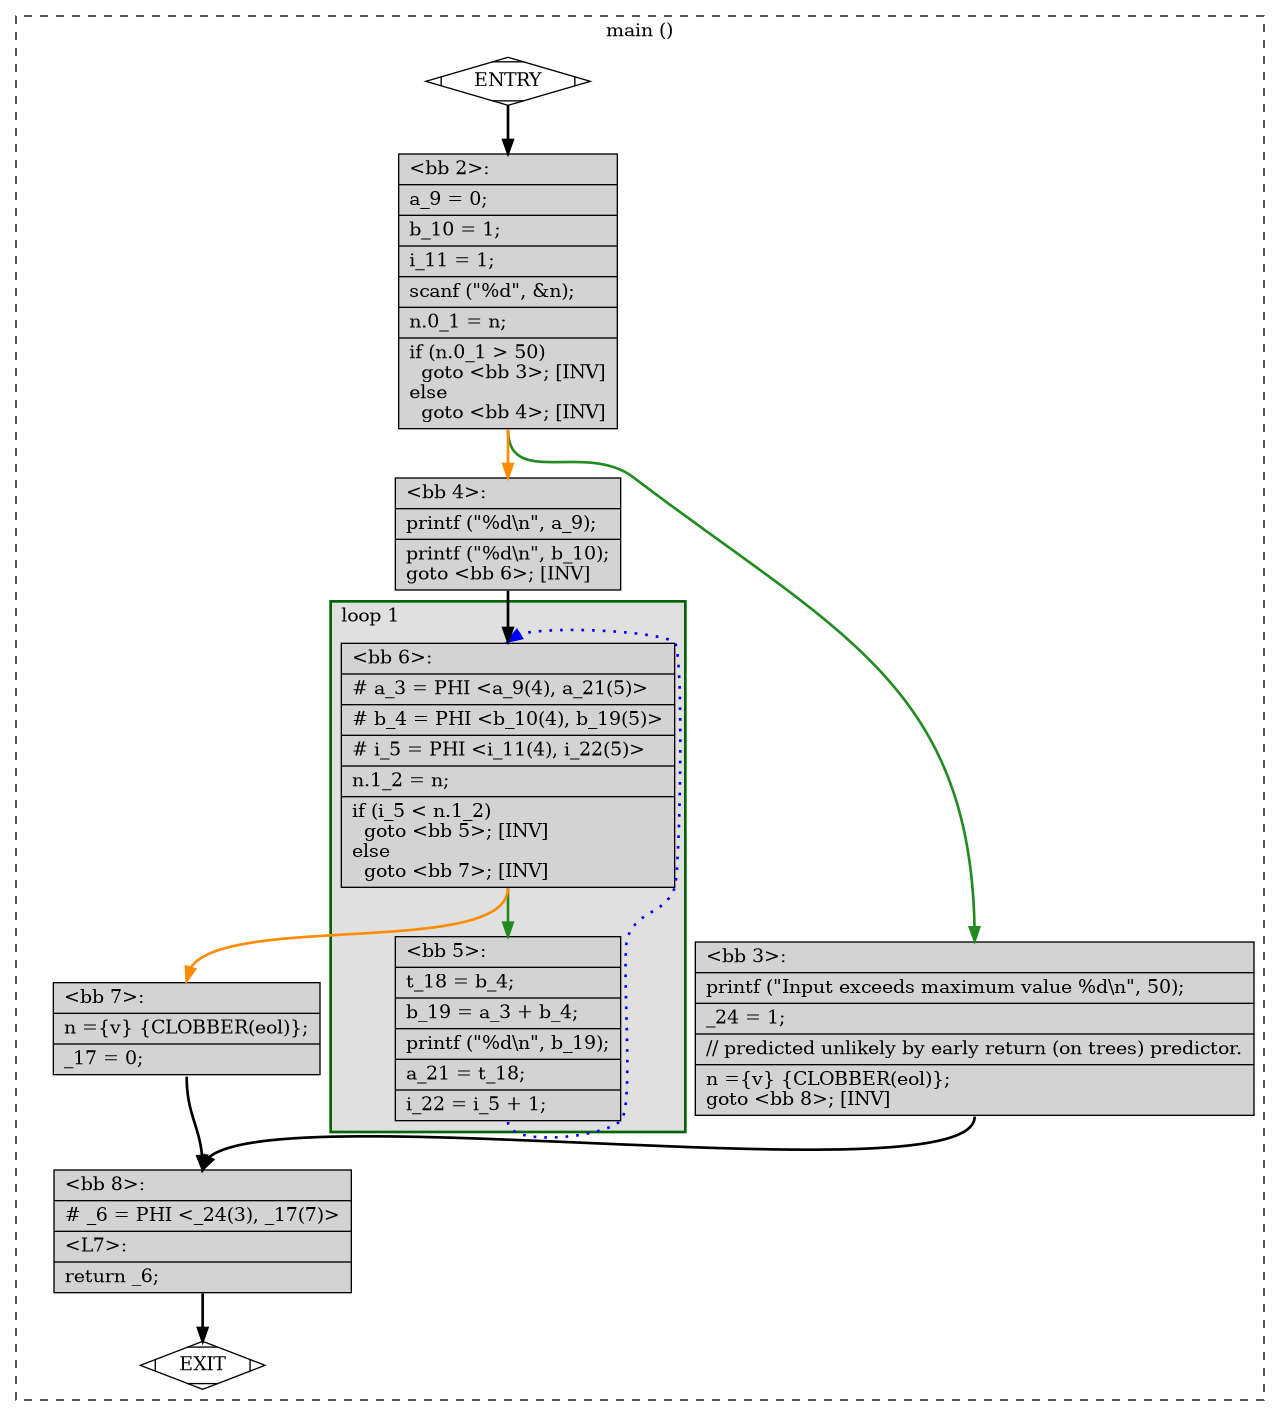
\includegraphics[width=0.5\linewidth]{ccl_7.png}
    \caption{cfg03.png/cfg04.png (029t/094t)}
    \label{fig:placeholder}
\end{figure}

结果表明,015t和020t、029t和094t这两对阶段之间的CFG是完全一致的,所以变化发生在020t至029t阶段之间。观察到主要变化有两点:
\begin{itemize}
    \item 有一些需要初始化数值的变量被添加了进来;
    \item 几乎所有的参数名被修改,特点是都被标记上了各不相同的编号(有些非变量的标识符也被标记了)。
\end{itemize}

根据上面的发现,推测这一部分是进行了分析上的进阶。原先,仅仅分析全局的逻辑,不考虑具体参量的赋值,特别是初始赋值。分析进阶后,将所有变量的赋值加入考虑,同时为了区分各个参量,类似于给所有变量/标识符赋予独特的ID,用以在后续的分析过程中更清晰地区分各个变量。

\vspace{1em}

通过上面的分析,切实地观察到了中间代码将AST翻译成中间表示的动态过程。编译器的\textbf{中间代码生成阶段功能验证完毕}。

\subsubsection{代码优化}
\texttt{\large{代码优化:主要工作是在不改变程序语义前提下,提升代码运行效率、缩减代码体积,让生成的代码\textbf{更快、更小或更省能}。}}

\vspace{1em}

在LLVM框架下,优化和分析都是通过 \textbf{Pass }进行的。官方将Pass分为以下三类:
\begin{enumerate}
    \item \textbf{Analysis Pass:} 不直接修改代码,只是收集信息,供其他 Pass 使用。一般从中可以分析出代码整体的逻辑架构,各种分支结构等等。
    \item \textbf{Transform Pass:} 对代码进行改造与优化。具体的有如,\textbf{常量传播}(比如\texttt{x = 1 + 2}直接传播为\texttt{x = 3}),\textbf{死代码删除}(永远不会执行或无副作用的代码),循环优化(这又包含\textbf{循环展开}、\textbf{循环不变代码外提}等),\textbf{内联优化},公共子表达式消除等。
    \item \textbf{Utility Passes:} 辅助操作,不属于纯粹的分析或优化,但在 IR 处理时提供支持功能。例子有,IR 打印、统计信息输出,Pass 管理相关的功能等。
\end{enumerate}

如果想要观察优化过程中代码本身的变化,可以执行以下命令:
\begin{center}
    \textcolor{deepblue}{\textbf{\texttt{\large{llc -print-before-all -print-after-all main.ll > main.log 2>\&1}}}}
\end{center}

这句命令调用了 LLVM 的 llc 工具。\texttt{-print-before-all}和\texttt{-print-after-all}参数分别用于指示打印出\textbf{每个 Pass 之前和之后的状态}用来观察与分析。\texttt{> main.log}意为将结果输出为该文件。\texttt{2>\&1}表示把 \textbf{标准错误} 也重定向到 \textbf{标准输出},则所有输出(包括错误信息、调试信息)都会显示在输出文件\texttt{main.log}中。

执行此命令之后,将会产生文件\texttt{main.log},里面包含了每个 LLVM Pass 之前/之后状态的所有信息。\texttt{main.log}文件长达数万行,不便于一一分析,此处选取一个明显的变化细节作简单阐述。

在原日志文件中第875行之前,每一轮都存在这样一个语句:
\begin{lstlisting}[frame=trbl,language={C++}]
br i1 %20, label %21, label %31
\end{lstlisting}

它的含义是,循环条件为假时,直接跳到基本块 \%31。

而从此算起的下一轮中,在第931行,这一语句被修改为:
\begin{lstlisting}[frame=trbl,language={C++}]
br i1 %20, label %21, label %.loopexit
\end{lstlisting}

这表明,LLVM 引入了一个新的块 \texttt{.loopexit}. 这一变化是 \textbf{loop-simplify pass/循环优化Pass} 的一个重要步骤,它确保每个循环都有\textbf{唯一的退出块},从而便于后续优化(如循环展开、强度削减)。

\vspace{1em}

除了通过上面命令输出 LLVM Passes 的具体日志,还可以直接使用不同的编译优化选项来探索优化过程对于代码效率的影响。

注意,此过程需要使用\hyperref[we-talked-about-it-here]{\textbf{\textcolor{deepblue}{在之前}}}提及到的\texttt{.bc}格式文件(LLVM bitcode 二进制文件)。从 LLVM IR 的\texttt{.ll}文件生成\texttt{.bc}文件的命令如下:
\begin{center}
    \textcolor{deepblue}{\textbf{\texttt{\large{llvm-as main.ll -o main.bc}}}}
\end{center}

有了\texttt{.bc}文件之后就可以根据需要,改变编译优化选项参数来生成新的\texttt{.ll}文件,例如:
\begin{center}
    \textcolor{deepblue}{\textbf{\texttt{\large{opt -S -O1 main.bc -o main-O1.ll}}}}
\end{center}
就生成了\texttt{O1}编译优化的LLVM IR. 后续再从\texttt{.ll}文件出发进行汇编、链接等步骤就可以生成最终优化后的程序。

\vspace{1em}

为了对比不同编译优化选项下程序的性能,需要进行计时作为对比参量。将原来的程序进行如下的修改,使其能够完整记录运行时:
\begin{lstlisting}[title=修改后的 main.c,frame=trbl,language={C++}]
#include <stdio.h>
#include <stdlib.h>
#include <sys/time.h>

#define MAX_N 100
#define INIT_A 0
#define INIT_B 1

#define PRINT(x) printf("%d\n", x)

int main() {
    int a, b, i, t, n;
    struct timeval start, end;
    double elapsed;

    a = INIT_A;
    b = INIT_B;
    i = 1;

    // time start
    gettimeofday(&start, NULL);

    PRINT(a);
    PRINT(b);

    // this is a friendly annotation *
    while (i < n)
    {
        t = b;
        b = a + b;
        PRINT(b);
        a = t;
        i = i + 1;
    }

    // time end
    gettimeofday(&end, NULL);

    // calculate
    elapsed = (end.tv_sec - start.tv_sec) + (end.tv_usec - start.tv_usec) / 1000000.0;

    printf("Execution time: %.6f seconds\n", elapsed);

}
\end{lstlisting}

因为后续测试数据可能很大(不考虑实际运行的数理正确性,只考虑运行效能),删除了输入数据的越界判断处理。

修改后,生成各个优化选项下的最终可执行文件完整命令行过程如下图所示:
\begin{figure} [H]
    \centering
    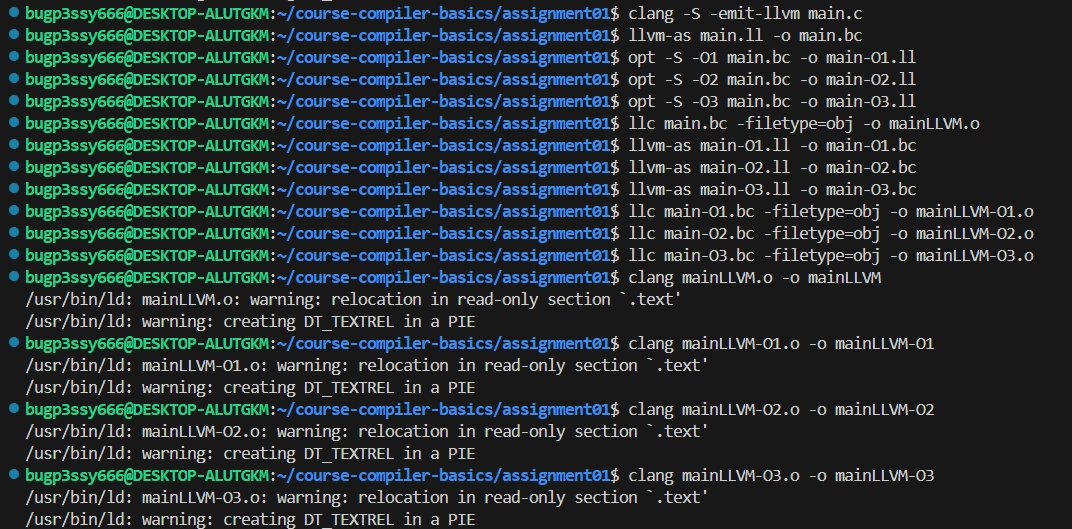
\includegraphics[width=0.75\linewidth]{ccl_0.jpg}
    \caption{优化程序生成过程}
    \label{fig:placeholder}
\end{figure}

最后,在此目录下依次运行各可执行文件,得到如下的运行时结果:
\begin{figure} [H]
    \centering
    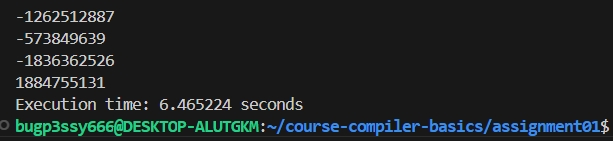
\includegraphics[width=0.7\linewidth]{ccl_1.jpg}
    \caption{无编译优化}
    \label{fig:placeholder}
\end{figure}

\begin{figure} [H]
    \centering
    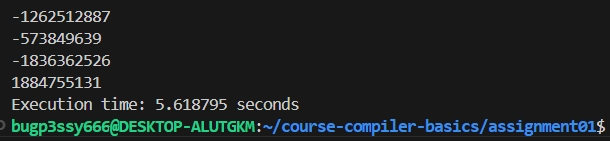
\includegraphics[width=0.7\linewidth]{ccl_2.jpg}
    \caption{-O1 编译优化}
    \label{fig:placeholder}
\end{figure}

\begin{figure} [H]
    \centering
    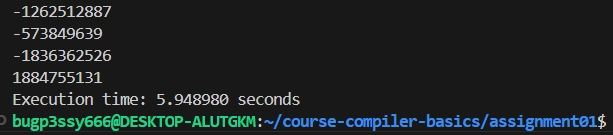
\includegraphics[width=0.7\linewidth]{ccl_3.jpg}
    \caption{-O2 编译优化}
    \label{fig:placeholder}
\end{figure}

\begin{figure} [H]
    \centering
    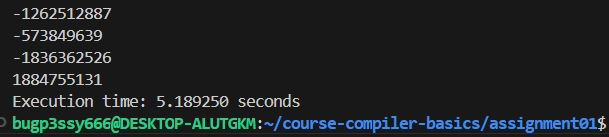
\includegraphics[width=0.7\linewidth]{ccl_4.jpg}
    \caption{-O3 编译优化}
    \label{fig:placeholder}
\end{figure}

实际上,可能由于本机性能问题等,运行时并不稳定,上面的数据只是在相对稳定时截取。但从数据中可以明确观察到的是,\textbf{采用编译优化选项的程序确实相较于无编译优化的程序有运行速度上的提升}。

\vspace{1em}

至此,编译器的\textbf{代码优化阶段功能验证完毕}。


\subsubsection{代码生成}
\texttt{\large{代码生成:以中间语言或预处理后文件为输入,生成目标语言(汇编语言)。}}

\vspace{1em}

对于x86、ARM、LLVM,分别执行下面的命令生成对应的汇编代码:

\begin{center}
    \textcolor{deepblue}{\textbf{\texttt{\large{gcc main.i -S -o mainx86.S}}}}
\end{center}

\begin{center}
    \textcolor{deepblue}{\textbf{\texttt{\large{aarch64-linux-gnu-gcc main.i -S -o mainARM.S}}}}
\end{center}

\begin{center}
    \textcolor{deepblue}{\textbf{\texttt{\large{llc main.ll -o mainLLVM.S}}}}
\end{center}

生成结果都是\texttt{.S}文件。

\vspace{1em}

\subsection{汇编器}
\subsubsection{汇编器的具体功能}
\textbf{汇编器} 接受汇编语言源程序(上面生成的\texttt{.S}文件),将其转化为目标机器代码的\textbf{目标文件}(\texttt{.o}文件),为二进制格式。

具体工作包括:
\begin{enumerate}
    \item \textbf{词法/语法分析:} 与编译器类似地,汇编器也需要读源代码,把汇编指令、伪指令、标号、注释等进行词法/语法解析,确认代码符合目标架构的汇编语法。
    \item \textbf{符号收集:} 进行第一遍扫描,收集汇编代码中的\textbf{符号}(label)和\textbf{外部引用}(extern),进行相应的标记或记录。
    \item \textbf{指令和伪指令翻译:} 进行第二遍扫描,把助记符(如 \texttt{mov, add, jmp})翻译成对应的机器指令编码,并处理伪指令。
    \item \textbf{地址与重定位信息生成:} 汇编器不能完全确定所有地址(例如调用外部函数),所以会生成 \textbf{重定位信息},供链接器处理。
    \item \textbf{生成目标文件(\texttt{.o})。}
\end{enumerate}

对于x86、ARM、LLVM的汇编代码,分别执行下面的命令,将其转化为目标文件:
\begin{center}
    \textcolor{deepblue}{\textbf{\texttt{\large{gcc mainx86.S -c -o mainx86.o}}}}
\end{center}

\begin{center}
    \textcolor{deepblue}{\textbf{\texttt{\large{aarch64-linux-gnu-gcc mainARM.S -c -o mainARM.o}}}}
\end{center}

\begin{center}
    \textcolor{deepblue}{\textbf{\texttt{\large{llc main.bc -filetype=obj -o mainLLVM.o}}}}
\end{center}

生成各自的\texttt{.o}目标文件。

\subsubsection{反汇编与汇编程序分析}
通过反汇编,可以得到与目标文件对应的原始汇编代码。此处仅对x86进行分析,执行下面的代码:
\begin{center}
    \textcolor{deepblue}{\textbf{\texttt{\large{objdump -d mainx86.o}}}}
\end{center}

执行后,汇编代码会直接在终端输出。输出结果如下,已经逐行进行分析并作注释:
\begin{lstlisting}[title=mainx86.o 反汇编结果与分析,frame=trbl,language={[x86masm]Assembler}]
0000000000000000 <main>:
   0:   f3 0f 1e fa             endbr64
                              ; CET 指令:用于控制流完整性,与逻辑无关
   4:   55                      push   %rbp
                              ; 保存旧的基指针
   5:   48 89 e5                mov    %rsp,%rbp
                              ; rbp = rsp,建立新的栈帧基址
   8:   48 83 ec 20             sub    $0x20,%rsp
                              ; 栈分配 32 字节局部空间(局部变量和对齐)
   c:   64 48 8b 04 25 28 00    mov    %fs:0x28,%rax
  13:   00 00 
                              ; 读取线程局部存储的值,用于栈保护
  15:   48 89 45 f8             mov    %rax,-0x8(%rbp)
                              ; 将值存到栈帧的 -0x8(%rbp)(在函数返回时检验)
  19:   31 c0                   xor    %eax,%eax
                              ; eax 置零,用于设置返回值或清零寄存器
  1b:   c7 45 e8 00 00 00 00    movl   $0x0,-0x18(%rbp)
                              ; a = 0
  22:   c7 45 ec 01 00 00 00    movl   $0x1,-0x14(%rbp)
                              ; b = 1
  29:   c7 45 f0 01 00 00 00    movl   $0x1,-0x10(%rbp)
                              ; i = 1
  30:   48 8d 45 e4             lea    -0x1c(%rbp),%rax
                              ; 为 scanf 准备 n 的地址
  34:   48 89 c6                mov    %rax,%rsi
                              ; rsi = &n,scanf 的第二个参数
  37:   48 8d 05 00 00 00 00    lea    0x0(%rip),%rax        # 3e <main+0x3e>
  3e:   48 89 c7                mov    %rax,%rdi
                              ; "%d" 的地址,通过重定位填充
  41:   b8 00 00 00 00          mov    $0x0,%eax
                              ; eax 置零,varargs 调用约定
  46:   e8 00 00 00 00          call   4b <main+0x4b>
                              ; 调用函数 scanf("%d", &n)
  4b:   8b 45 e4                mov    -0x1c(%rbp),%eax
                              ; 取出 scanf 写入的 n 赋给 eax
  4e:   83 f8 32                cmp    $0x32,%eax
                              ; 判断 if (n > 50)
  51:   7e 20                   jle    73 <main+0x73>
                              ; 若 eax <= 50 则跳到 address 0x73(处理正常路径),否则继续 n > 50 的分支
  53:   be 32 00 00 00          mov    $0x32,%esi
                              ; 将常数 50 放到 esi,作为 printf 的参数
  58:   48 8d 05 00 00 00 00    lea    0x0(%rip),%rax        # 5f <main+0x5f>
  5f:   48 89 c7                mov    %rax,%rdi
                              ; 准备 scanf 字符串参数地址
  62:   b8 00 00 00 00          mov    $0x0,%eax
                              ; eax 置零,可变参数调用约定
  67:   e8 00 00 00 00          call   6c <main+0x6c>
                              ; 调用 printf,打印越界字符串信息
  6c:   b8 01 00 00 00          mov    $0x1,%eax
                              ; 返回值 eax = 1(准备作为 main 函数返回值)
  71:   eb 70                   jmp    e3 <main+0xe3>
                              ; 跳转到函数结尾处做清理和返回
  73:   8b 45 e8                mov    -0x18(%rbp),%eax
                              ; 处于正常路径:eax = a,准备打印 a
  76:   89 c6                   mov    %eax,%esi
                              ; a 赋给 esi(printf 第二个参数)
  78:   48 8d 05 00 00 00 00    lea    0x0(%rip),%rax        # 7f <main+0x7f>
  7f:   48 89 c7                mov    %rax,%rdi
                              ; 准备字符串参数地址
  82:   b8 00 00 00 00          mov    $0x0,%eax
  87:   e8 00 00 00 00          call   8c <main+0x8c>
                              ; printf("%d\n", a);
  8c:   8b 45 ec                mov    -0x14(%rbp),%eax
                              ; eax = b,准备打印 b,下同理
  8f:   89 c6                   mov    %eax,%esi
  91:   48 8d 05 00 00 00 00    lea    0x0(%rip),%rax        # 98 <main+0x98>
  98:   48 89 c7                mov    %rax,%rdi
  9b:   b8 00 00 00 00          mov    $0x0,%eax
  a0:   e8 00 00 00 00          call   a5 <main+0xa5>
                              ; printf("%d\n", b);
  a5:   eb 2f                   jmp    d6 <main+0xd6>
                              ; 打印完 a,b 之后跳到循环判断处、
  a7:   8b 45 ec                mov    -0x14(%rbp),%eax        ; 循环体起始行
                              ; eax = b
  aa:   89 45 f4                mov    %eax,-0xc(%rbp)
                              ; t = b 
  ad:   8b 45 e8                mov    -0x18(%rbp),%eax
                              ; eax = a 
  b0:   01 45 ec                add    %eax,-0x14(%rbp)
                              ; b = a + b 
  b3:   8b 45 ec                mov    -0x14(%rbp),%eax
                              ; eax = b,再次准备打印......
  b6:   89 c6                   mov    %eax,%esi
  b8:   48 8d 05 00 00 00 00    lea    0x0(%rip),%rax        # bf <main+0xbf>
  bf:   48 89 c7                mov    %rax,%rdi
  c2:   b8 00 00 00 00          mov    $0x0,%eax
  c7:   e8 00 00 00 00          call   cc <main+0xcc>
                              ; printf("%d\n", b) ,输出此轮 b
  cc:   8b 45 f4                mov    -0xc(%rbp),%eax
                              ; eax = t 
  cf:   89 45 e8                mov    %eax,-0x18(%rbp)
                              ; a = t 
  d2:   83 45 f0 01             addl   $0x1,-0x10(%rbp)
                              ; 循环计数参量 i 的累加
  d6:   8b 45 e4                mov    -0x1c(%rbp),%eax
                              ; eax = n 
  d9:   39 45 f0                cmp    %eax,-0x10(%rbp)
                              ; 等同于 cmp n, i,比较 n 与 i 大小
  dc:   7c c9                   jl     a7 <main+0xa7>
                              ; 如果 n < i ,跳回循环体 a7 继续循环计算
  de:   b8 00 00 00 00          mov    $0x0,%eax
                              ; 否则循环结束,设 main 返回值 eax = 0
  e3:   48 8b 55 f8             mov    -0x8(%rbp),%rdx
                              ; 将起始时栈上保存的值读入 rdx
  e7:   64 48 2b 14 25 28 00    sub    %fs:0x28,%rdx
  ee:   00 00 
                              ; rdx = rdx - [fs:0x28]
                              ; 比较保存值与当前 TLS canary
  f0:   74 05                   je     f7 <main+0xf7>
                              ; 如果相等(即没有栈破坏),跳到 f7 正常返回
  f2:   e8 00 00 00 00          call   f7 <main+0xf7>
                              ; 如果不等,调用特定函数异常处理
  f7:   c9                      leave
                              ; 恢复栈帧: mov rsp, rbp; pop rbp ...
  f8:   c3                      ret
                              ; 返回

\end{lstlisting}

通过分析汇编代码,可以看到程序在栈、内存层面上的一些细节操作。总体分析下来,代码逻辑和原始的C源码是一致的。

\vspace{1em}

\textbf{汇编器功能验证完毕}。

\vspace{1em}

\subsection{链接器}
链接器把编译器/汇编器产生的若干\textbf{目标文件}(.o)、\textbf{静态库}(.a)与\textbf{共享库}(.so)合并,做各种符号处理、地址修正、布局修缮等工作,输出最终的\textbf{目标文件}或可执行镜像,并为运行时装载留下必要的元数据。

具体的链接流程包括:
\begin{enumerate}
    \item \textbf{输入收集:} 读取命令行给定的 object 文件、静态库、共享库,对静态库按需展开。
    \item \textbf{符号/节汇总:} 为每个输入文件构建\textbf{符号表}和\textbf{节}(有如\texttt{.text,.data,.bss,.rodata,} 重定位节等),并合并相同类型的节。
    \item \textbf{地址分配:} 分配每个输出节的\textbf{虚拟地址}(VMA)和\textbf{文件偏移}(LMA),设置段对齐、分页规则、加载段划分等。
    \item \textbf{符号解析:} 对每个\textbf{未定义}符号找到“最合适”的替换定义,此外处理强/弱符号优先级、重复定义、符号可见性等问题。
    \item \textbf{重定位的生成/处理:} 把对地址的占位修正为最终地址或产生需要运行时修正的信息,分为\textbf{静态重定位}和\textbf{动态重定位}两种。
    \item \textbf{写入输出文件:} 编写目标文件/\textbf{可执行文件},包含节、段、符号表、重定位条目、动态节等字段。
\end{enumerate}

对于x86,ARM和LLVM在汇编器中转化得到的目标文件,分别用下面的指令进行链接:
\begin{center}
    \textcolor{deepblue}{\textbf{\texttt{\large{gcc mainx86.o -o mainx86}}}}
\end{center}

\begin{center}
    \textcolor{deepblue}{\textbf{\texttt{\large{aarch64-linux-gnu-gcc -o mainARM mainARM.o -static -lc}}}}
\end{center}

\begin{center}
    \textcolor{deepblue}{\textbf{\texttt{\large{clang mainLLVM.o -o mainLLVM}}}}
\end{center}

执行后得到没有后缀的\textbf{可执行文件}。

\texttt{.o} 目标文件和最终生成的可执行文件都是不可直接阅读的二进制文件,且这一部分不是最主要的学习内容,故不作进一步研究。

\vspace{1em}

\subsection{运行程序}
经过以上各个步骤,已经得到了x86,ARM和LLVM的最终可执行文件。由于处在Ubuntu的Linux虚拟环境下,直接在当前目录下打开就可以验证程序功能(ARM需要qemu运行):
\begin{figure} [H]
    \centering
    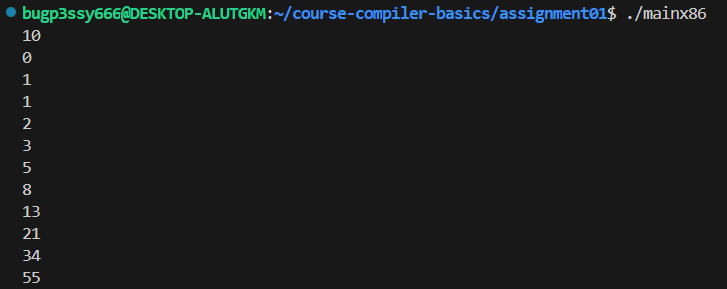
\includegraphics[width=0.75\linewidth]{run_1.png}
    \caption{x86的可执行文件运行结果}
    \label{fig:placeholder}
\end{figure}

\begin{figure} [H]
    \centering
    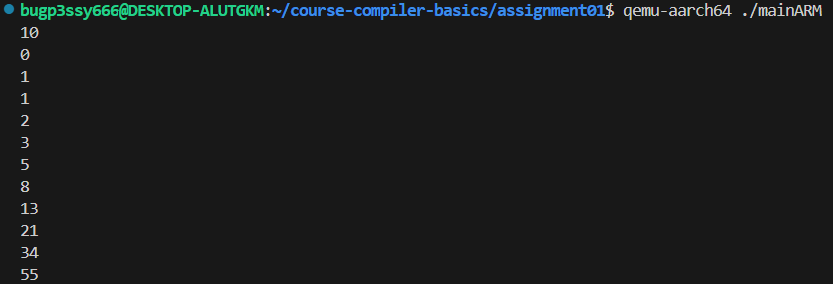
\includegraphics[width=0.75\linewidth]{res_arm.png}
    \caption{ARM的可执行文件运行结果}
    \label{fig:placeholder}
\end{figure}

\begin{figure}[H]
    \centering
    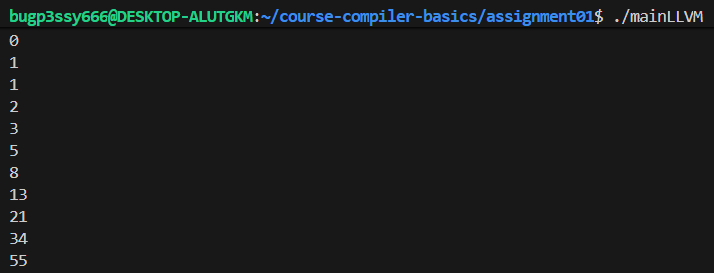
\includegraphics[width=0.75\linewidth]{run_2.png}
    \caption{LLVM的可执行文件运行结果}
    \label{fig:placeholder}
\end{figure}

对于三个可执行程序,均用测试数据10进行测试,都得到正确的输出数字串。说明程序本身逻辑正确,且以上经过的各个处理阶段均没有产生错误。

\vspace{2em}

\textbf{\large{至此,实验一全部完成。}}

%——————————————————————————————————————

\vspace{3em}

\section{实验二:LLVM IR编程}

\subsection{SysY程序编写} \label{this-subsection}

首先在第二问中我们小组等价的SysY程序如下:

\begin{lstlisting}
#include <stdio.h>

int max(int a, int b);
int factorial(int n);

int main() {
	int a = 10;
	int b = 5;
	int result = 0;
	int i = 0;
	int n = 5;

	result = a + b;
	result = a - b;  
	result = a * b;
	printf("%d\n", result);
	result = a / b;
	result = a % b;

	result = a;
	result = result + 1;
	result = result * 2;
	printf("%d\n", result);

	if (a > b) {
		result = 1;
	} else {
		result = 0;
	}

	if (a > 0 && b > 0) {
		result = 1;
	}

	if (a > 0 || b > 0) {
		result = 1;
	}

	if (a > b) {
		result = max(a, b);
	} else if (a < b) {
		result = b;
	} else {
		result = 0;
	}

	printf("%d\n", result);
	i = 0;
	result = 0;
	while (i <= 10) {
		result = result + i;
		i = i + 1;
	}

	result = 0;
	for (i = 0; i < 10; i = i + 1) {
		if (i % 2 == 0) {    
			continue;
		}
		result = result + i;

		if (result > 20) {
			break;
		}
	}

	result = factorial(n);
	printf("%d\n", result);

	int arr[5] = {1, 2, 3, 4, 5};
	arr[0] = 10;
	result = arr[0] + arr[1];
	printf("%d\n", result);

	return 0;
}

int max(int a, int b) {
	if (a > b) {
		return a;
	} else {
		return b;
	}
}

int factorial(int n) {
	if (n <= 1) {
		return 1;
	} else {
		return n * factorial(n - 1);
	}
}
\end{lstlisting}

上述代码包含了编译器支持的大部分语句操作(包括数值运算,赋值语句,分支语句,循环语句,函数定义和调用等),运行结果如下图:
\begin{figure}[H]
	\centering
	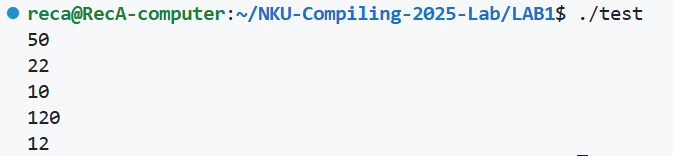
\includegraphics[width=10cm]{expected_res.png}
	\caption{源SysY程序运行结果}
\end{figure}

下面展示我们小组完成的与上述程序等价的LLVM IR程序和ARM汇编程序。

\vspace{1em}

\subsection{LLVM IR编程}

强博负责的LLVM IR的编程,完成的等价程序如下:

\begin{lstlisting}
@.str = private unnamed_addr constant [4 x i8] c"%d\0A\00", align 1

declare i32 @printf(ptr noundef, ...) #1

;定义函数max
define dso_local i32 @max(i32 noundef %0, i32 noundef %1) #0 {
	%3 = alloca i32, align 4
	%4 = alloca i32, align 4
	%5 = alloca i32, align 4
	store i32 %0, ptr %4, align 4
	store i32 %1, ptr %5, align 4
	%6 = load i32, ptr %4, align 4
	%7 = load i32, ptr %5, align 4
	%8 = icmp sgt i32 %6, %7
	br i1 %8, label %9, label %11

9:                                                
	%10 = load i32, ptr %4, align 4
	store i32 %10, ptr %3, align 4
	br label %13

11:                                             
	%12 = load i32, ptr %5, align 4
	store i32 %12, ptr %3, align 4
	br label %13

13:                                               
	%14 = load i32, ptr %3, align 4
	ret i32 %14
}

; 定义函数factorial
define dso_local i32 @factorial(i32 noundef %0) #0 {
	%2 = alloca i32, align 4
	%3 = alloca i32, align 4
	store i32 %0, ptr %3, align 4
	%4 = load i32, ptr %3, align 4
	%5 = icmp sle i32 %4, 1
	br i1 %5, label %6, label %7

6:                                          
	store i32 1, ptr %2, align 4
	br label %13

7:                                            
	%8 = load i32, ptr %3, align 4
	%9 = load i32, ptr %3, align 4
	%10 = sub nsw i32 %9, 1
	%11 = call i32 @factorial(i32 noundef %10)
	%12 = mul nsw i32 %8, %11
	store i32 %12, ptr %2, align 4
	br label %13

13:                                           
	%14 = load i32, ptr %2, align 4
	ret i32 %14
}

;定义主函数
define dso_local i32 @main() #0 {
	;定义临时变量
	%1 = alloca i32, align 4
	%2 = alloca i32, align 4
	%3 = alloca i32, align 4
	%4 = alloca i32, align 4
	%5 = alloca i32, align 4
	%6 = alloca i32, align 4
	%7 = alloca [5 x i32], align 16
	;变量赋值初始化
	store i32 0, ptr %1, align 4
	store i32 10, ptr %2, align 4
	store i32 5, ptr %3, align 4
	store i32 0, ptr %4, align 4
	store i32 0, ptr %5, align 4
	store i32 5, ptr %6, align 4

	; 执行result = a + b
	%8 = load i32, ptr %2, align 4
	%9 = load i32, ptr %3, align 4
	%10 = add nsw i32 %8, %9
	store i32 %10, ptr %4, align 4

	; 执行result = a - b
	%11 = load i32, ptr %2, align 4
	%12 = load i32, ptr %3, align 4
	%13 = sub nsw i32 %11, %12
	store i32 %13, ptr %4, align 4

	; 执行result = a * b
	%14 = load i32, ptr %2, align 4
	%15 = load i32, ptr %3, align 4
	%16 = mul nsw i32 %14, %15
	store i32 %16, ptr %4, align 4

	; 执行printf("%d\n", result)
	%17 = load i32, ptr %4, align 4
	%18 = call i32 (ptr, ...) @printf(ptr noundef @.str, i32 noundef %17)

	; 执行result = a / b
	%19 = load i32, ptr %2, align 4
	%20 = load i32, ptr %3, align 4
	%21 = sdiv i32 %19, %20
	store i32 %21, ptr %4, align 4

	; 执行result = a % b
	%22 = load i32, ptr %2, align 4
	%23 = load i32, ptr %3, align 4
	%24 = srem i32 %22, %23
	store i32 %24, ptr %4, align 4

	; 执行result = a
	%25 = load i32, ptr %2, align 4
	store i32 %25, ptr %4, align 4

	; 执行result = result + 1
	%26 = load i32, ptr %4, align 4
	%27 = add nsw i32 %26, 1
	store i32 %27, ptr %4, align 4

	; 执行result = result * 2
	%28 = load i32, ptr %4, align 4
	%29 = mul nsw i32 %28, 2
	store i32 %29, ptr %4, align 4

	; 执行printf("%d\n", result)
	%30 = load i32, ptr %4, align 4
	%31 = call i32 (ptr, ...) @printf(ptr noundef @.str, i32 noundef %30)

	; 实现分支判断if (a > b)
	%32 = load i32, ptr %2, align 4
	%33 = load i32, ptr %3, align 4
	%34 = icmp sgt i32 %32, %33
	br i1 %34, label %35, label %36

35:                                               
	store i32 1, ptr %4, align 4
	br label %37

36:                                               
	store i32 0, ptr %4, align 4
	br label %37

37:                                               
	; 执行分支判断if (a > 0 && b > 0)
	%38 = load i32, ptr %2, align 4
	%39 = icmp sgt i32 %38, 0
	br i1 %39, label %40, label %44

40:                                               
	%41 = load i32, ptr %3, align 4
	%42 = icmp sgt i32 %41, 0
	br i1 %42, label %43, label %44

43:                                               
	store i32 1, ptr %4, align 4
	br label %44

44:                                              
	; 执行分支判断if (a > 0 || b > 0)
	%45 = load i32, ptr %2, align 4
	%46 = icmp sgt i32 %45, 0
	br i1 %46, label %50, label %47

47:
	%48 = load i32, ptr %3, align 4
	%49 = icmp sgt i32 %48, 0
	br i1 %49, label %50, label %51

50:
	store i32 1, ptr %4, align 4
	br label %51

51:
	; 执行多重分支判断if (a > b) ... else if (a < b) ... else ...
	%52 = load i32, ptr %2, align 4
	%53 = load i32, ptr %3, align 4
	%54 = icmp sgt i32 %52, %53
	br i1 %54, label %55, label %59

55:
	%56 = load i32, ptr %2, align 4
	%57 = load i32, ptr %3, align 4
	%58 = call i32 @max(i32 noundef %56, i32 noundef %57)
	store i32 %58, ptr %4, align 4
	br label %67

59:
	%60 = load i32, ptr %2, align 4
	%61 = load i32, ptr %3, align 4
	%62 = icmp slt i32 %60, %61
	br i1 %62, label %63, label %65

63:
	%64 = load i32, ptr %3, align 4
	store i32 %64, ptr %4, align 4
	br label %66

65:
	store i32 0, ptr %4, align 4
	br label %66

66: 
	br label %67

67:
	; 执行printf("%d\n", result)
	%68 = load i32, ptr %4, align 4
	%69 = call i32 (ptr, ...) @printf(ptr noundef @.str, i32 noundef %68)

	; 执行赋值语句i = 0和result = 0
	store i32 0, ptr %5, align 4
	store i32 0, ptr %4, align 4
	br label %70

70:
	; 实现循环while (i <= 10)
	%71 = load i32, ptr %5, align 4
	%72 = icmp sle i32 %71, 10
	br i1 %72, label %73, label %80

73:
	; 执行result和i的自增
	%74 = load i32, ptr %4, align 4
	%75 = load i32, ptr %5, align 4
	%76 = add nsw i32 %74, %75
	store i32 %76, ptr %4, align 4
	%77 = load i32, ptr %5, align 4
	%78 = add nsw i32 %77, 1
	store i32 %78, ptr %5, align 4
	br label %70, !llvm.loop !6

79:
	br label %80

80:                                               
	store i32 0, ptr %4, align 4
	; 实现循环for (i = 0; i < 10; i = i + 1)
	store i32 0, ptr %5, align 4
	br label %81

81:                                          
	%82 = load i32, ptr %5, align 4
	%83 = icmp slt i32 %82, 10
	br i1 %83, label %84, label %106

84:
	;实现分支if (i % 2 == 0)                                   
	%85 = load i32, ptr %5, align 4
	%86 = srem i32 %85, 2
	%87 = icmp eq i32 %86, 0
	br i1 %87, label %88, label %89

88:                                              
	br label %100

89:                                            
	; 执行result = result + i
	%90 = load i32, ptr %4, align 4
	%91 = load i32, ptr %5, align 4
	%92 = add nsw i32 %90, %91
	store i32 %92, ptr %4, align 4
	; 实现分支if (result > 20) break
	%93 = load i32, ptr %4, align 4
	%94 = icmp sgt i32 %93, 20
	br i1 %94, label %95, label %96

95:                                               
	br label %106

96:                                               
	br label %97

97:                                               
	br label %98

98:                                              
	br label %99

99:                                               
	br label %100

100:                                           
	; 实现i自增
	%101 = load i32, ptr %5, align 4
	%102 = add nsw i32 %101, 1
	store i32 %102, ptr %5, align 4
	br label %81, !llvm.loop !8

103:                                              
	br label %81

104:                                              
	br label %105

105:                                             
	br label %106

106:                                             
	; 函数调用 factorial(n)
	%107 = load i32, ptr %6, align 4
	%108 = call i32 @factorial(i32 noundef %107)
	store i32 %108, ptr %4, align 4
	%109 = load i32, ptr %4, align 4
	%110 = call i32 (ptr, ...) @printf(ptr noundef @.str, i32 noundef %109)

	; 实现数组赋值int arr[5] = {1, 2, 3, 4, 5};
	%111 = getelementptr inbounds [5 x i32], ptr %7, i64 0, i64 0
	store i32 1, ptr %111, align 16
	%112 = getelementptr inbounds [5 x i32], ptr %7, i64 0, i64 1
	store i32 2, ptr %112, align 4
	%113 = getelementptr inbounds [5 x i32], ptr %7, i64 0, i64 2
	store i32 3, ptr %113, align 8
	%114 = getelementptr inbounds [5 x i32], ptr %7, i64 0, i64 3
	store i32 4, ptr %114, align 4
	%115 = getelementptr inbounds [5 x i32], ptr %7, i64 0, i64 4
	store i32 5, ptr %115, align 16

	; 实现数组元素赋值arr[0] = 10
	%116 = getelementptr inbounds [5 x i32], ptr %7, i64 0, i64 0
	store i32 10, ptr %116, align 16

	%117 = getelementptr inbounds [5 x i32], ptr %7, i64 0, i64 0
	%118 = load i32, ptr %117, align 16
	%119 = getelementptr inbounds [5 x i32], ptr %7, i64 0, i64 1
	%120 = load i32, ptr %119, align 4
	%121 = add nsw i32 %118, %120
	store i32 %121, ptr %4, align 4

	%122 = load i32, ptr %4, align 4
	%123 = call i32 (ptr, ...) @printf(ptr noundef @.str, i32 noundef %122)

	ret i32 0
}

!llvm.module.flags = !{!0, !1, !2, !3, !4}
!llvm.ident = !{!5}

!0 = !{i32 1, !"wchar_size", i32 4}
!1 = !{i32 8, !"PIC Level", i32 2}
!2 = !{i32 7, !"PIE Level", i32 2}
!3 = !{i32 7, !"uwtable", i32 2}
!4 = !{i32 7, !"frame-pointer", i32 2}
!5 = !{!"Ubuntu clang version 18.1.3 (1ubuntu1)"}
!6 = distinct !{!6, !7}
!7 = !{!"llvm.loop.mustprogress"}
!8 = distinct !{!8, !7}
\end{lstlisting}

使用命令:clang -o mytest test\_llvm.ll libsysy\_x86.a和lli -load=./sylib.so test\_llvm.ll进行验证,最终上述test\_llvm.ll程序进行编译链接后运行结果如下图:

\begin{figure}[H]
	\centering
	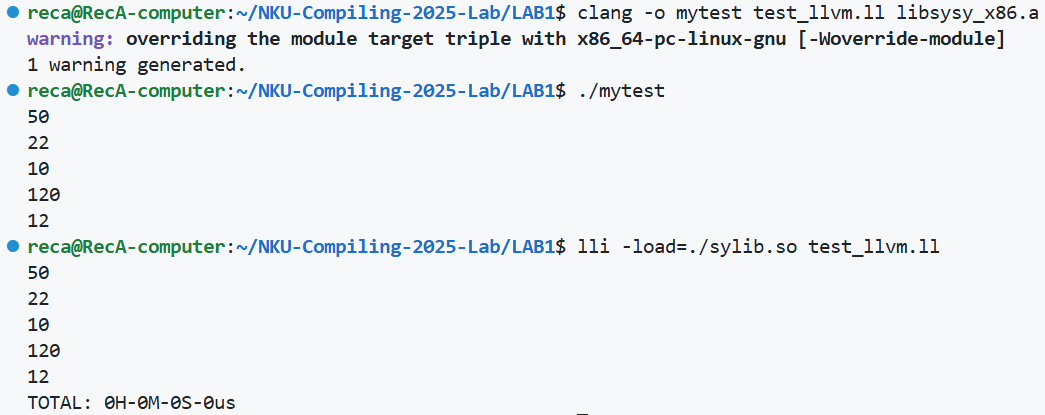
\includegraphics[width=10cm]{mytest-result.png}
	\caption{等价LLVM程序运行结果}
\end{figure}

下面,对LLVM编写的程序中的各语言特性进行说明:

\begin{itemize}
	\item 局部变量的声明均以\%开头表示虚拟寄存器,并使用alloca关键字为其分配对应的内存空间,i32表示的是局部变量的数据类型是32位整型变量。
	\item 数组类型的变量声明使用“alloca [5 x i32]”表示数组元素个数位5,类型为i32。访问数组元素时需要使用getelementptr关键字,以语句“\%116 = getelementptr inbounds [5 x i32], ptr \%7, i64 0, i64 0”为例,[5 x i32]表示将计算具有5个i32元素的数组的地址,基址为ptr \%7,后面的两个索引中第二个表示要访问元素的下标。
	\item 函数定义使用define关键字,由于本程序均为全局函数,所以函数名前都用@修饰,调用函数时使用call关键字,后面接函数返回类型、函数名和实参列表。函数结束后使用关键字ret实现返回功能
	\item 分支控制语句和循环语句实现的关键是使用br关键字实现跳转,可以用于无条件跳转也可以用于条件跳转。
	\item 本程序实现的算数运算符有+,-,*,/,\%,其对应的关键字分别为add,sub, mul, sdiv,srem。实现关系运算需要声明关键字icmp,后面紧跟需要实现的关系运算,包括小于(slt)、大于(sgt)、小于等于(sle)、等于(eq)等。
\end{itemize}

%——————————————————————————————————————
\vspace{3em}

\section{实验三:ARM 汇编编程}
\begin{center}
	\texttt{注:陈语童(2311887)负责此实验的代码编写、探究和报告撰写。}
\end{center}

\vspace{1em}

为了更全面地探究编译器支持的SysY语言特性,编写了全新的SysY程序,用于上面一节的LLVM IR程序实验探究,和本节的ARM汇编程序实验探究。

\subsection{SysY程序}
新的完整的SysY程序已经在\hyperref[this-subsection]{\textbf{\textcolor{deepblue}{~3.1~节~}}}中给出。

此SysY程序所涉及到的语言特性,全面涵盖了赋值、数值运算的基本操作,条件分支、循环等复合语句,数组的声明和调用,以及自定义函数的特性。

直接编译该SysY程序,得到下面的输出:
\begin{figure} [H] \label{expectation}
    \centering
    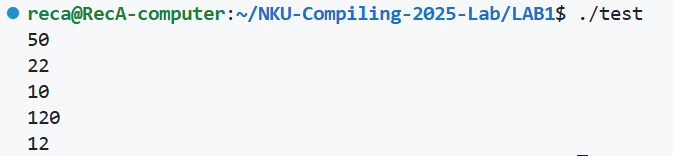
\includegraphics[width=0.7\linewidth]{expected_res.png}
    \caption{预期输出结果}
    \label{fig:placeholder}
\end{figure}

则最终编写的汇编程序在经过汇编器转化和最后的链接加载后得到的可执行程序,运行后也应该得到这样的结果。

\vspace{1em}

\subsection{ARM 汇编代码设计过程}
下面按照自然代码顺序,分块阐述ARM汇编代码设计过程。

\vspace{1em}

首先必须明确的是,ARM汇编中的寄存器编码与x86不同。32寄存器系\texttt{w0, w1, ... },64寄存器系\texttt{x0, x1, ...},编写时需注意与x86区分、寄存器之间区分。

\vspace{1em}

汇编文件起始,先参考了前面斐波那契数列生成的ARM汇编语言代码,按照规则编写文件头,并全局地声明了一个必要的字面常量:
\begin{lstlisting}[frame=trbl,language={[x86masm]Assembler}]
	.arch armv8-a
	.file	"example.c"
    
	.text
	.section	.rodata
	.align	3
.LC1:
	.string	"%d\n"
\end{lstlisting}

其中\texttt{.arch armv8-a}指明架构是 ARMv8-A (AArch64),\texttt{.rodata}表示只读数据段,后面声明一个用于\texttt{printf()}函数中的常量字符串参数\texttt{"\%d\textbackslash n"},\texttt{LC}表示字面常量。

\begin{lstlisting}[frame=trbl,language={[x86masm]Assembler}]
	.global	main
	.type	main, %function
main:
\end{lstlisting}

进入 \texttt{main} 函数。

\begin{lstlisting}[frame=trbl,language={[x86masm]Assembler}]
	sub	sp, sp, #80            ; 在栈上分配 80 字节空间
	stp	x29, x30, [sp, 64]     ; 保存前一帧的帧指针和返回地址
	add	x29, sp, 64            ; 设置新的帧指针
\end{lstlisting}

为函数创建栈帧的基本操作。得到栈的结构大致如下所示:

\begin{lstlisting}[frame=trbl]
sp+0   → 临时变量
sp+12  → 用于存放中间结果
sp+16  → 其他局部变量
...
sp+64  → 保存 x29
sp+72  → 保存 x30
\end{lstlisting}

\vspace{1em}

\begin{lstlisting}[frame=trbl,language={[x86masm]Assembler}]
mov	w0, 10
str	w0, [sp, 20]
mov	w0, 5
str	w0, [sp, 24]
str	wzr, [sp, 12]
str	wzr, [sp, 16]
mov	w0, 5
str	w0, [sp, 28]
\end{lstlisting}

这一部分与\textbf{赋值}的语言特性有关。观察之前工作过程中ARM汇编语言代码,发现与x86会汇编语言不同的是,可以使用\texttt{[基址, 偏移量]}的格式来指示地址,较为方便。此处就采用这样的写法。其中\texttt{mov, str}分别是ARM中数据移动和寄存器中数据写入内存地址的汇编指令。这一部分对应原SysY代码的:

\begin{lstlisting}[frame=trbl,language={C}]
    int a = 10;     
    int b = 5;
    int result = 0;
    int i = 0;
    int n = 5;
\end{lstlisting}

\vspace{1em}

下面三段汇编代码与基本\textbf{四则运算}的语言特性有关。

\begin{lstlisting}[frame=trbl,language={[x86masm]Assembler}]
ldr	w1, [sp, 20]
ldr	w0, [sp, 24]
add	w0, w1, w0
str	w0, [sp, 12]
\end{lstlisting}

第一段是\texttt{result = a + b;}对应的运算。\texttt{ldr}是\texttt{str}的逆操作,将数据从内存中读取到寄存器中。\texttt{add}则显然易见地是将两个操作数相加存入目标寄存器中的指令。那么上面编写的汇编指令意义就是,先将\texttt{a, b}的数据分别读取到寄存器中,再将两个寄存器的值相加存到其中一个寄存器中作为结果,最后再将这个结果寄存器的数值写入内存地址,对应的是\texttt{result}变量的地址。


\begin{lstlisting}[frame=trbl,language={[x86masm]Assembler}]
ldr	w1, [sp, 20]
ldr	w0, [sp, 24]
sub	w0, w1, w0
str	w0, [sp, 12]
\end{lstlisting}

第二段是\texttt{result = a - b;}对应的运算。基本原理一致,这次使用到\texttt{sub}减法操作。可以发现三次读取/写入数据的地址和上面加法中是完全一致的,则\texttt{result}的值在这个过程中被不可逆地覆盖。

\begin{lstlisting}[frame=trbl,language={[x86masm]Assembler}]
ldr	w1, [sp, 20]
ldr	w0, [sp, 24]
mul	w0, w1, w0
str	w0, [sp, 12]
\end{lstlisting}

第三段是\texttt{result = a * b}对应的运算。ARM中也有直接的\texttt{mul}乘法操作。

\vspace{1em}

\begin{lstlisting}[frame=trbl,language={[x86masm]Assembler}]
ldr	w1, [sp, 12]
adrp	x0, .LC1
add	x0, x0, :lo12:.LC1
bl	printf
\end{lstlisting}

这里涉及到对上面计算结果的\textbf{输出},也是SysY语言一大特性。

第一行,将要打印的数加载到第二参数上;第二行和第三行共同作用将之前标记为\texttt{.LC1}的字符串常量\texttt{"\%d\textbackslash n"}加载到第一参数上;最后一行通过\texttt{bl}指令(带链接的跳转),直接跳转到外部函数\texttt{printf}进行输出。

后续调用自定义的函数时,也可以直接使用\texttt{bl}进行跳转。其中字符串常量的加载中,\texttt{adrp}只将\texttt{.L1}标签的页面的基地址加载到 \texttt{x0} 寄存器,通过下一语句的加法,\texttt{.LC1}标签的低12位偏移量被加和到 \texttt{x0} 上,才完成完整地址的计算,指向目标字符常量。

接下来还有除法和取余的运算,和上面四则运算的基本原理相同。但值得注意的是,取余运算没有直接的指令符,需要拆分成“除法→乘法→减法”三步,才能计算出余数:

\begin{lstlisting}[frame=trbl,language={[x86masm]Assembler}]
ldr	w0, [sp, 20]
ldr	w1, [sp, 24]
sdiv	w2, w0, w1          ; 先做整除法,向下取整
ldr	w1, [sp, 24]
mul	w1, w2, w1          ; 乘法,计算出已经被整除的部分
sub	w0, w0, w1          ; 减法,减去已被整除的部分得到余数
str	w0, [sp, 12]
\end{lstlisting}

此后的自增与左移都能够直接或间接地通过单条运算指令来解决,不再单独展示。

\vspace{1em}

下面展示部分\textbf{条件判断}语句的编写。

\begin{lstlisting}[frame=trbl,language={[x86masm]Assembler}]
ldr	w1, [sp, 20]
ldr	w0, [sp, 24]
cmp	w1, w0
ble	.L2
mov	w0, 1
str	w0, [sp, 12]
b	.L3
.L2:
str	wzr, [sp, 12]
.L3:
··· ··· ··· ···
\end{lstlisting}


条件判断的逻辑起点是比较。使用\texttt{cmp}进行两个数的比较,这里是对\texttt{a, b}两个参量比较。之后来到判断之后分支逻辑的核心,\texttt{ble}表示小于等于时跳转,\texttt{b}表示无条件跳转。从源代码分支逻辑的分析出发,关键区别在于不同情况下给\texttt{result}赋的值不同,那么就需要利用跳转将这一分支实现,两个赋值语句在两种情况下均为“有其中一条语句被执行而另一条不被执行的状态”。所以选择用\texttt{.L2}标签隔离不满足条件时的赋值语句,同时用\texttt{b}指令保证满足条件时跳过被隔离的赋值语句。此外还需要注意的点是,赋零不能直接用数字0,而要用\texttt{\#0}立即数0,或者像这里的编写一样,使用\texttt{wzr}零寄存器来赋值,更高效与保险。综上,这段汇编代码能够成功复现下面原SysY代码中的条件分支:

\begin{lstlisting}[frame=trbl,language={C}]
    if (a > b) {
        result = 1;
    } else {
        result = 0;
    }
\end{lstlisting}

再往后分析一个代表性条件分支。

\begin{lstlisting}[frame=trbl,language={[x86masm]Assembler}]
ldr	w0, [sp, 20]
cmp	w0, 0
ble	.L4
ldr	w0, [sp, 24]
cmp	w0, 0
ble	.L4
mov	w0, 1
str	w0, [sp, 12]
.L4:
··· ··· ··· ···
\end{lstlisting}

这里的条件分支中有双重条件。思路是,只要有一个条件不被满足,就直接跳转到不满足条件的后续逻辑。所以,在上面编写的代码可以看到,两次\texttt{cmp}之后都进行了\texttt{ble}的判断是否跳转。如果两次都满足——都没有跳转,才能执行到\texttt{.L4}标签前的那一段赋值操作。这段汇编代码能够复现下面原SysY代码中的条件分支:

\begin{lstlisting}[frame=trbl,language={C}]
    if (a > 0 && b > 0) {
        result = 1;
    }
\end{lstlisting}

此后条件分支的汇编翻译过程大同小异,最多只是进行进一步的逻辑嵌套,不再赘述。

\vspace{1em}

下面再简单分析一下怎么写\textbf{循环语句}块的ARM汇编代码。

\begin{lstlisting}[frame=trbl,language={[x86masm]Assembler}]
str	wzr, [sp, 12]
str	wzr, [sp, 16]
b	.L10
.L11:
··· ··· ··· ···         ; 循环内部的实际逻辑
.L10:
ldr	w0, [sp, 16]
cmp	w0, 10
ble	.L11
\end{lstlisting}

一般在每一次循环之后,进行条件的复查,判断是否需要继续进行下一轮循环。所以判断逻辑理所应当地排布在循环体实际内容之后,并且在循环实际内容的开头设置标签,方便判断后的跳转。但初始状态,也需要进行一次判断,所以像上面汇编代码中所示,将判断部分也要单独进行标签标记,第一次到达循环体前跳转到判断逻辑进行初次判断,这样才符合原代码逻辑。上面实现的循环在原SysY代码中是这样的:

\begin{lstlisting}[frame=trbl,language={C}]
    while (i <= 10) {       
        ··· ··· ··· ···     // 实际循环内容
    }
\end{lstlisting}

for循环的实现是同理的,不再介绍如何编写。

\vspace{1em}

在源程序的主函数最后,还进行了\textbf{数组的声明和赋值}。

\begin{lstlisting}[frame=trbl,language={[x86masm]Assembler}]
.LC0:
	.word	1
	.word	2
	.word	3
	.word	4
	.word	5
\end{lstlisting}

数组的声明,在主函数之后单独编写。其中\texttt{.LC0}为这里的数组进行字符常量的唯一标识;5个\texttt{.word}是声明32位(4字节)的数据的作用,即\texttt{int}类型数据,后面跟随的是实际数值。所以上面的声明用SysY写出来就是


\begin{lstlisting}[frame=trbl,language={[x86masm]Assembler}]
adrp	x0, .LC0
add	x0, x0, :lo12:.LC0
add	x2, sp, 32
mov	x3, x0
ldp	x0, x1, [x3]
stp	x0, x1, [x2]
ldr	w0, [x3, 16]
str	w0, [x2, 16]
\end{lstlisting}

实际主函数中,并不能直接使用声明的字符常量数组,而要将其全部复制形成一个新的可以修改值的数组。上面的汇报代码中,前两行之前分析过,是获得字符常量实际地址的作用。下面分配新的数组在栈上的位置,并保存前面获得的字符常量数组地址。后面四行是数组复制的一个以缩减代码量、提高效率的写法。\texttt{ldp}和\texttt{stp}都能够一次读取/加载16字节数据,那么为了获得一个5项32位数据,只需要两组操作即可(一次移动16字节=16*8位=4项),第二组操作进行16字节的偏移即可。

因此,\texttt{int arr[5] = {1, 2, 3, 4, 5};}这一句声明语句不仅需要在主函数后声明常量,还需要写如上的汇编语句将其复制为可操作的局部变量。

后续对于数组数据的修改,和之前将数据直接存储到内存是一个道理,不再赘述了。

\vspace{1em}

示例SysY程序还尝试编写了\textbf{自定义函数},函数逻辑主体应该写在主函数结束后。
\begin{lstlisting}[frame=trbl,language={[x86masm]Assembler}]
	.global	max
	.type max, %function
max:
    cmp w0, w1
    ble .L22
    ret
.L22:
    mov w0, w1
    ret
\end{lstlisting}

先看\texttt{max}较大值函数。首先进行一些设置,\texttt{.global}表示全局函数全局可用;\texttt{\%function}声明这是一个函数。下面进行两个传入参数的大小比较,如果满足条件,默认返回\texttt{w0}对应的参数值;否则将另一参数赋给\texttt{w0}寄存器并返回值。

\begin{lstlisting}[frame=trbl,language={[x86masm]Assembler}]
	.global	factorial
	.type	factorial, %function
factorial:
	stp	x29, x30, [sp, -32]!
	mov	x29, sp
	str	w0, [sp, 28]
	ldr	w0, [sp, 28]
	cmp	w0, 1
	bgt	.L23
	mov	w0, 1
	b	.L24
.L23:
	ldr	w0, [sp, 28]
	sub	w0, w0, #1
	bl	factorial
	mov	w1, w0
	ldr	w0, [sp, 28]
	mul	w0, w1, w0
.L24:
	ldp	x29, x30, [sp], 32
	ret
\end{lstlisting}

再看\texttt{factorial}阶乘函数,此函数涉及到递归。头部声明不再解析。最开始几行做简单的栈帧分配操作,并将传入的参数\texttt{n}入栈。接下来用\texttt{cmp}和\texttt{bgt}(如果大于跳转)组合做\texttt{n <= 1}的比较,处理0和1的阶乘直接返回1. 而如果大于1则跳转到\texttt{.L23}进行递归处理(对应\texttt{else}语句块),易理解接下来的代码在进行下面几件事:计算\texttt{n - 1},以计算得到的\texttt{n - 1}参数递归地调用\texttt{factorial}函数,将递归结果与\texttt{n}相乘并作为返回结果。

在所有用到栈的函数体最后,都需要清理和恢复栈帧。对于本程序,\texttt{main}函数和\texttt{factorial}函数都用到了栈帧,所以需要依次做如下操作:

\begin{lstlisting}[frame=trbl,language={[x86masm]Assembler}]
; function: main
	ldp	x29, x30, [sp, 64]
	add	sp, sp, 80
	ret
; function: factorial
.L24:
	ldp	x29, x30, [sp], 32
	ret
\end{lstlisting}

由于篇幅限制不能够逐行解析汇编代码的编写,但未展示的部分与已经分析的部分基本逻辑相近,故不再赘述。

\vspace{1em}

\subsection{ARM 汇编代码综合展示}
为了节省报告篇幅,完整的ARM汇编代码不在此处直接展示。

敬请直接跳转到 GitHub 仓库阅读:\href{https://github.com/bugp3ssy666/NKU-compiler-basics/blob/main/Lab0/example-SysY/exampleARM.S}{exampleARM.S}

\vspace{1em}

\subsection{正确性验证}

将代码用以下的指令进行汇编处理和链接加载,获得最终的可执行文件:
\begin{figure} [H]
    \centering
    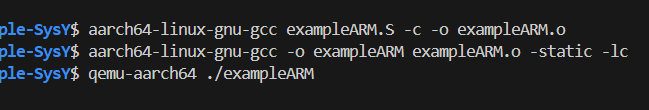
\includegraphics[width=0.75\linewidth]{load_process.png}
    \caption{获得可执行文件}
    \label{fig:placeholder}
\end{figure}

使用qemu运行ARM可执行文件:

\begin{figure} [H]
    \centering
    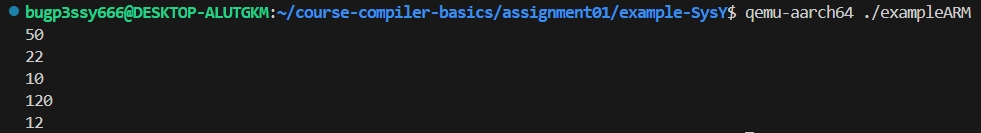
\includegraphics[width=0.85\linewidth]{runtime_result.jpg}
    \caption{运行结果}
    \label{fig:placeholder}
\end{figure}

可以看到,这和之前的预期输出结果(\hyperref[expectation]{图17})是完全一致的。

\vspace{1em}

\subsection{思考与启发}
将高级语言翻译成汇编语言是一个很复杂的过程,因为两者基本逻辑不同。高级语言顺着人自然思考的范式而展开,汇编语言则需要根据机器运行的顺序依次指示。而且汇编语言自由度低,不能够像高级语言那样几乎是随心所欲地重命名参数、函数,比如寄存器等名称是既定不可更改的,会给程序的编写带来一定困惑。

然而编写过程中也感受到,相对于x86的汇编语言,ARM汇编语言似乎能编写地更加美观和简洁,受益于简单易懂的标准参数名称、指令名称,以及一些便捷的逻辑表达方式,比如访存时的方括号格式。

在此之前我修读过汇编语言这门课程,以上的实验让我温故而知新,对于汇编语言有了更深刻的了解和认识。

\vspace{1em}

\textbf{\large{至此,实验三全部完成。}}

%——————————————————————————————————————


%----------------------------------------------------------------
\vspace{3em}

\section{总结}
本次实验是课程后续主要实验的前置实验,着重分析探究了编译流程和编译器各阶段功能,并进行了 LLVM IR 中间代码程序和 ARM 汇编代码程序的编写。

在实验一中,从理论出发,用各种 Clang/GCC 等命令,将 C 语言程序从\texttt{.c}源文件,到中间语言程序文件、汇编语言程序文件、机器码文件,再到最终的可执行文件这一完整编译过程完整走了一遍。在这当中,主要分析了编译器各个阶段做的工作,并进行了机器进程操作层面的前后代码对比,尽可能深入地探究其功能。

在实验三中,根据之前的汇编语言知识和阅读经验,尝试编写和优化 SysY 程序的等价 ARM 汇编语言。结果是成功的,运行后得到了预期结果。在汇编语言的编写过程中,对其有了语法语义上的更深一步了解,并且能够与其他汇编语言联想对比,分析 ARM 汇编语言的特性。

\vspace{2em}

\textbf{实验代码的 GitHub 仓库:}

陈语童(2311887):\href{https://github.com/bugp3ssy666/NKU-compiler-basics/tree/main/Lab0}{NKU-compiler-basics/Lab0}

强博(2313825):\href{https://github.com/RecA123/NKU-Compiling-2025-Lab/tree/main/LAB1}{NKU-Compiling-2025-Lab/LAB1}

%--------------------------------------------------------------
\end{document}
